%% bare_conf_compsoc.tex
%% V1.4b
%% 2015/08/26
%% by Michael Shell
%% See:
%% http://www.michaelshell.org/
%% for current contact information.
%%
%% This is a skeleton file demonstrating the use of IEEEtran.cls
%% (requires IEEEtran.cls version 1.8b or later) with an IEEE Computer
%% Society conference paper.
%%

% Edited for the paper on DP properties of quantum recommendation algorithm, to be submitted to S&P 2024.
% No redistribution of this version.

\documentclass[conference,compsoc]{IEEEtran}
% Some/most Computer Society conferences require the compsoc mode option,
% but others may want the standard conference format.
%
% If IEEEtran.cls has not been installed into the LaTeX system files,
% manually specify the path to it like:
% \documentclass[conference,compsoc]{../sty/IEEEtran}

% Some very useful LaTeX packages include:
% (uncomment the ones you want to load)

% *** CITATION PACKAGES ***
%
\ifCLASSOPTIONcompsoc
  % IEEE Computer Society needs nocompress option
  % requires cite.sty v4.0 or later (November 2003)
  \usepackage[nocompress]{cite}
\else
  % normal IEEE
  \usepackage{cite}
\fi
% cite.sty was written by Donald Arseneau
% V1.6 and later of IEEEtran pre-defines the format of the cite.sty package
% \cite{} output to follow that of the IEEE. Loading the cite package will
% result in citation numbers being automatically sorted and properly
% "compressed/ranged". e.g., [1], [9], [2], [7], [5], [6] without using
% cite.sty will become [1], [2], [5]--[7], [9] using cite.sty. cite.sty's
% \cite will automatically add leading space, if needed. Use cite.sty's
% noadjust option (cite.sty V3.8 and later) if you want to turn this off
% such as if a citation ever needs to be enclosed in parenthesis.
% Note that some packages require special options to format as the Computer
% Society requires. In particular, Computer Society  papers do not use
% compressed citation ranges as is done in typical IEEE papers
% (e.g., [1]-[4]). Instead, they list every citation separately in order
% (e.g., [1], [2], [3], [4]). To get the latter we need to load the cite
% package with the nocompress option which is supported by cite.sty v4.0
% and later.
\usepackage{lipsum}         % testing
\usepackage[utf8]{inputenc} % allow utf-8 input
\usepackage[T1]{fontenc}    % use 8-bit T1 fonts
\usepackage{hyperref}       % hyperlinks
\usepackage{url}            % simple URL typesetting
\usepackage{booktabs}       % professional-quality tables
\usepackage{amsfonts}       % blackboard math symbols
\usepackage{nicefrac}       % compact symbols for 1/2, etc.
\usepackage{microtype}      % microtypography
\usepackage{xcolor}         % colors
\usepackage{amsmath}
\usepackage{amssymb}
\usepackage{xfrac}
\usepackage{caption}
\usepackage{float}
\usepackage{lscape}
\usepackage{bm}
\usepackage{multirow}
\usepackage{algorithm}
\usepackage{algorithmicx}
\usepackage{algpseudocode}
\usepackage{tikz}
\usepackage[all]{xy}
\usetikzlibrary{calc}

\ifCLASSOPTIONcompsoc
 \usepackage[caption=false,font=footnotesize,labelfont=sf,textfont=sf]{subfig}
\else
 \usepackage[caption=false,font=footnotesize]{subfig}
\fi
% subfig.sty, written by Steven Douglas Cochran, is the modern replacement
% for subfigure.sty, the latter of which is no longer maintained and is
% incompatible with some LaTeX packages including fixltx2e. However,
% subfig.sty requires and automatically loads Axel Sommerfeldt's caption.sty
% which will override IEEEtran.cls' handling of captions and this will result
% in non-IEEE style figure/table captions. To prevent this problem, be sure
% and invoke subfig.sty's "caption=false" package option (available since
% subfig.sty version 1.3, 2005/06/28) as this is will preserve IEEEtran.cls
% handling of captions.
% Note that the Computer Society format requires a sans serif font rather
% than the serif font used in traditional IEEE formatting and thus the need
% to invoke different subfig.sty package options depending on whether
% compsoc mode has been enabled.
%
% The latest version and documentation of subfig.sty can be obtained at:
% http://www.ctan.org/pkg/subfig

% *** FLOAT PACKAGES ***
%
%\usepackage{fixltx2e}
% fixltx2e, the successor to the earlier fix2col.sty, was written by
% Frank Mittelbach and David Carlisle. This package corrects a few problems
% in the LaTeX2e kernel, the most notable of which is that in current
% LaTeX2e releases, the ordering of single and double column floats is not
% guaranteed to be preserved. Thus, an unpatched LaTeX2e can allow a
% single column figure to be placed prior to an earlier double column
% figure.
% Be aware that LaTeX2e kernels dated 2015 and later have fixltx2e.sty's
% corrections already built into the system in which case a warning will
% be issued if an attempt is made to load fixltx2e.sty as it is no longer
% needed.
% The latest version and documentation can be found at:
% http://www.ctan.org/pkg/fixltx2e

%\usepackage{stfloats}
% stfloats.sty was written by Sigitas Tolusis. This package gives LaTeX2e
% the ability to do double column floats at the bottom of the page as well
% as the top. (e.g., "\begin{figure*}[!b]" is not normally possible in
% LaTeX2e). It also provides a command:
%\fnbelowfloat
% to enable the placement of footnotes below bottom floats (the standard
% LaTeX2e kernel puts them above bottom floats). This is an invasive package
% which rewrites many portions of the LaTeX2e float routines. It may not work
% with other packages that modify the LaTeX2e float routines. The latest
% version and documentation can be obtained at:
% http://www.ctan.org/pkg/stfloats
% Do not use the stfloats baselinefloat ability as the IEEE does not allow
% \baselineskip to stretch. Authors submitting work to the IEEE should note
% that the IEEE rarely uses double column equations and that authors should try
% to avoid such use. Do not be tempted to use the cuted.sty or midfloat.sty
% packages (also by Sigitas Tolusis) as the IEEE does not format its papers in
% such ways.
% Do not attempt to use stfloats with fixltx2e as they are incompatible.
% Instead, use Morten Hogholm'a dblfloatfix which combines the features
% of both fixltx2e and stfloats:

% correct bad hyphenation here
%\hyphenation{op-tical net-works semi-conduc-tor}

%预定义命令
\newcommand{\degree}{^\circ}%摄氏度
\newcommand{\dd}{\mathrm{d}}%微分中的直立体d

% Define Dirac notation
\newcommand\bra[1]{\left\langle#1\right|}%左氏bra
\newcommand\ket[1]{\left|#1\right\rangle}%右矢ket
\newcommand\qinner[2]{\left\langle#1\right.\left|#2\right\rangle}%态矢量的内积
\newcommand\qouter[2]{\left|#1\right\rangle\left\langle#2\right|}%态矢量的外积

% Misc
\newcommand\td\tilde
\renewcommand\O{\mathcal{O}}
\newcommand\A{\mathcal{A}}
\newcommand\lek{_{\le k}}
% Probability related shortcuts
\newcommand\E{\mathbf{E}}
\newcommand\Var{\mathbf{Var}}
\newcommand\iid{\overset{\text{i.i.d.}}{\sim}}
\newcommand\qed{\hfill\ensuremath{\square}}

% Greek letter shortcuts
\renewcommand\l{\ell}
\renewcommand\a{\alpha}
\renewcommand\b{\beta}
\newcommand\g{\gamma}
\newcommand\sig{\sigma}
\newcommand\Sig{\Sigma}
\newcommand\s{\sigma}
\newcommand\eps{\varepsilon}

% Lin.Alg. related: shortcuts for matrix and vector
\renewcommand\vec[1]{\bm{#1}}% vector
\renewcommand\v[1]{\vec{#1}}
\newcommand\mat[1]{\bm{#1}}% matrix

\newcommand\ul{\v u_\l}
\newcommand\vl{\v v_\l}
\newcommand\uli{u_{\l i}}
\newcommand\vlj{v_{\l j}}

% Define useful math operators that are not predefined by latex
\DeclareMathOperator*{\tr}{tr}
\DeclareMathOperator*{\diag}{diag}
\DeclareMathOperator*{\rank}{rank}
\DeclareMathOperator*{\laspan}{span}
\DeclareMathOperator*{\argmin}{argmin}
\DeclareMathOperator*{\argmax}{argmax}
\DeclareMathOperator*{\poly}{poly}
\DeclareMathOperator*{\polylog}{polylog}
\DeclareMathOperator*{\image}{image}
\DeclareMathOperator*{\Prob}{Prob}

% Define environments
\newtheorem{lemma}{Lemma}
\newtheorem{definition}{Definition}
\newtheorem{observation}{Observation}
\newtheorem{assumption}{Assumption}
\newtheorem{proposition}{Proposition}
\newtheorem{theorem}{Theorem}
\newtheorem{corollary}{Corollary}

\begin{document}
%
% paper title
% Titles are generally capitalized except for words such as a, an, and, as,
% at, but, by, for, in, nor, of, on, or, the, to and up, which are usually
% not capitalized unless they are the first or last word of the title.
% Linebreaks \\ can be used within to get better formatting as desired.
% Do not put math or special symbols in the title.
\title{Differential Privacy of Quantum and\\Quantum-Inspired-Classical
Recommendation Algorithms}


% author names and affiliations
% use a multiple column layout for up to three different
% affiliations
\author{
%\IEEEauthorblockN{Anonymous Author(s)}
\IEEEauthorblockN{Chenjian Li}
\IEEEauthorblockA{
    Key Laboratory of System Software (Chinese Academy of Sciences)\\
    State Key Laboratory of Computer Science, Institute of Software\\
    Chinese Academy of Sciences, Beijing, China\\
    University of Chinese Academy of Sciences\\
    Email: licj@ios.ac.cn
}
\and
\IEEEauthorblockN{Mingsheng Ying}
\IEEEauthorblockA{
    Centre for Quantum Software and Information\\
    University of Technology Sydney, Australia\\
    Email: Mingsheng.Ying@uts.edu.au
}
}

%conference papers do not typically use \thanks and this command
%is locked out in conference mode. If really needed, such as for
%the acknowledgment of grants, issue a \IEEEoverridecommandlockouts
%after \documentclass

\maketitle

\begin{abstract}
  We analyze the DP (differential privacy) properties of the quantum recommendation algorithm\cite{q_recommend_sys} and the quantum-inspired-classical recommendation algorithm\cite{ewin_tang_ciq}.
  We discover that the quantum recommendation algorithm is a privacy curating mechanism on its own, requiring no external noise, which is different from traditional differential privacy mechanisms. In our analysis, a novel perturbation method tailored for SVD (singular value decomposition) and low-rank matrix approximation problems is introduced. Using the perturbation method and random matrix theory, we are able to derive that both the quantum and quantum-inspired-classical algorithms are $\big(\td\O\big(\frac 1n\big),\,\, \td\O\big(\frac{1}{\min\{m,n\}}\big)\big)$-DP under some reasonable restrictions, where $m$ and $n$ are numbers of users and products in the input preference database respectively. Nevertheless, a comparison shows that the quantum algorithm has better privacy preserving potential than the classical one.
\end{abstract}

% For peer review papers, you can put extra information on the cover
% page as needed:
% \ifCLASSOPTIONpeerreview
% \begin{center} \bfseries EDICS Category: 3-BBND \end{center}
% \fi
%
% For peerreview papers, this IEEEtran command inserts a page break and
% creates the second title. It will be ignored for other modes.
\IEEEpeerreviewmaketitle

\section{Introduction}
  Since the quantum algorithm for factoring was proposed by Shor \cite{shor_algo} in 1994, quantum computation has attracted considerable attention in both computer science and physics research communities. After many quantum algorithms with exponential speedup over classical counterparts have been proposed\cite{shor_algo,grover_algo,hhl_algo}, it became a question whether \textit{quantum machine learning} algorithms can exhibit exponential speedup over their classical counterparts.
  In 2019, Kerenidis et al. \cite{q_recommend_sys} proposed a quantum algorithm that can perform low-rank matrix reconstruction efficiently. When applied to recommendation systems, it exhibit exponential speedup over any classical counterparts available by the time, attracting much attention from the research community.
  However, inspired by the quantum algorithm, an efficient classical algorithm was later discovered \cite{ewin_tang_ciq}, cancelling the exponential runtime advantage of the quantum algorithm. Nevertheless, Kerenidis' quantum algorithm still has better polynomial runtime complexity.

  While much focus has been placed on the time complexity of the quantum recommendation algorithm and its classical counterpart, there have been very limited analysis on other aspects of these algorithms. To our best knowledge, no prior work has been done to analyze the privacy property of the quantum recommendation algorithm. In this work, we address this gap by analyzing the privacy property of both algorithms within the differential privacy framework\cite{dwork_algodpbook}, and find that the quantum recommendation algorithm not only preserves differential privacy, but has many other interesting properties as well.

  %TODO
  %Besides the remained polynomial speedup, the quantum recommendation algorithm
  %for example, as will be shown in this paper, it is a data-curating mechanism for protecting privacy in itself, even with no artificially noise added.

  % Since its original proposal\cite{dwork2006calibrating}, differential privacy has attracted much attention in the privacy and security research community and
  In recent years, differential privacy (DP for short)  \cite{dwork2006calibrating} has become a prominent framework to analyze privacy of  machine learning and AI problems. At first glance, DP and quantum computation seem to be very distant realms. However, some surprising relationship between them has been noticed recently   \cite{aaronsonGentleMeasurementQuantum2019,qdp_ying}.
  On one hand, DP typically employs a randomized data-curating mechanism (i.e.
  %usually a machine learning algorithm or
  a randomized algorithm specifically designed to curate data) that samples from an ambiguous distribution generated from input data. On the other hand, in %quantum computation or
  quantum machine learning algorithms, a quantum state is usually prepared before quantum measurement, which is, in its essence, random sampling from certain distribution generated from input data.  Furthermore, the fundamental principles of quantum mechanics guarantee the state is destroyed immediately after sampling, preventing unwanted information copy (see no-cloning theorem \cite{nielsen_chuang_qcqi}) or leaking. The nature is somewhat preventing quantum experimentalists from learning too much knowledge, protecting the "privacy" of quantum states. Such similarity has led researchers to % attempts have been made to
  examine the concept of DP in quantum computing \cite{qdp_ying, aaronsonGentleMeasurementQuantum2019}.

{\vskip 3pt}

  \textbf{Contributions of this paper}: The aim of this paper is to analyze the DP of the quantum recommendation algorithm \cite{q_recommend_sys} and the quantum-inspired-classical recommendation algorithm \cite{ewin_tang_ciq}. %First, we surprisingly discover that the quantum recommendation algorithm is a data-curating mechanism for protecting privacy in itself, even with no artificially noise added.
  The DP of an algorithm is usually measured by a pair of parameters $(\eps,\delta)$, where $\eps$ bounds the multiplicative difference of its output probabilities before and after a private record is added to a database, and $\delta$ bounds the corresponding additive difference \cite{dwork_algodpbook}. By introducing a novel perturbation method for SVD (singular value decomposition) and low-rank matrix perturbation problems, we are able to settle the DP parameters of both algorithms:
  %-differential privacy parameter of an algorithm. $\eps$ and $\delta $ are non-negative numbers indicating the privacy preserving ability of a given algorithm. The smaller value of $\eps$,$\delta$, the better privacy-preserving the algorithm is. These parameters enables us to analyze the privacy preserving ability of an algorithm quantitavely, and lies in the heart of both classical\cite{dwork_algodpbook} and quantum\cite{aaronsonGentleMeasurementQuantum2019} differential privacy. Within the quantum realm, previous work have calculated the $(\eps,\delta)$ parameter of quantum tomography\cite{aaronsonGentleMeasurementQuantum2019}, (a kind of procedure/algorithm that tries to recover the entire quantum state from many queries to the state). However, the DP parameters and properties of many quantum machine learning algorithms remain unclear and is awaiting to be calculated and analyzed.

  \begin{theorem}[Main Result Preview, Informal] In a recommendation system containing $m$ users and $n$ products, the quantum recommendation algorithm $\A_{\rm RQ}^k$  \cite{q_recommend_sys} and quantum-inspired-classical recommendation algorithm $\A_{\rm RC}^k$\cite{ewin_tang_ciq}
  preserves $\left(\td\O\big(\frac 1n\big),\,\, \td\O\big(\frac{1}{\min\{m,n\}}\big)\right)$-DP for typical users.
  \end{theorem}

  Furthermore, we discover that both algorithms possess a surprisingly property which is distinct from traditional privacy curating mechanisms. The quantum recommendation algorithm as well as the quantum-inspired-classical algorithm is \textit{in itself a curating mechanism} under certain assumptions, with no additional noise needed. For the quantum algorithm, nor are any explicit sampling process needed, as quantum measurement has naturally taken the job. This poses a sharp contrast against traditional curating mechanisms, which heavily depends on adding external noise to data to protect privacy. That is to say, the quantum and quantum-inspired-classical recommendation algorithms can be viewed as zero-computation-overhead curating mechanisms.

  Finally, we compare the quantum and quantum-inspired algorithms through the lens of privacy. While both algorithms share similar properties in general, there're still nuances that make them different. Our analysis show that the quantum algorithm has better privacy preserving potential and is less susceptible to possible adversaries.

  {\vskip 3pt}

  \textbf{Organization of the paper}: In section \ref{sec2:preliminaries}, we provide a brief introduction to the problem and its related fields, such as quantum computation and differential privacy. In section \ref{sec3:method}, we present our methods and techniques gathered from various fields that will be used to derive our main results. In section \ref{sec4:dp_res}, we present and prove our main results on differential privacy of the algorithms. Finally in section \ref{sec5:discuss}, we discuss the privacy properties of both algorithms that are not captured by our main result, make comparisons between both algorithms, and point out the limitations of our current work.

\section{Preliminaries}\label{sec2:preliminaries}

\subsection{Singular Value Decomposition}
  Singular value decomposition (SVD) plays a central role in both the quantum recommendation algorithm and our analysis on it. The singular value decomposition states that any rectangular matrix $A\in\mathbb C^{m\times n}$ can be decomposed as $A=U\Sig V^\dag$, where $U,V$ are $m\times m$ and  $n\times n$ unitary matrices respectively, and $\Sig$ is a rectangular diagonal matrix with $\Sig_{ii}=\sig_i$, where $\sig_1\ge \sig_2\cdots\sig_{\min\{m,n\}}\ge 0$ are singular values of $A$. When $A$ is real, $U$ and $V$ reduces to real orthogonal matrices, and the Hermitian conjugate $V^\dag$ becomes simply the real transpose $V^T$.

  Although the matrix form $A=U\Sig V^\dag$ of SVD is widely used, in our context it is more convenient to express the SVD in its vector form
  \begin{equation}
    A=\sum_{i=1}^{\min\{m,n\}}\sig_i \v u_i \v v_i^\dag
  \end{equation}
  where $\v u_i$ and $\v v_i$ are the $i$-th column vector of $U$ and $V$, respectively.
  When it is clear from the context, we will abbreviate $\sum_{i=1}^{\min\{m,n\}}$ as $\sum_i$. Furthermore, we define the low-rank approximation of $A$ via SVD as $A_{\le k}:=\sum_{i=1}^k\sig_i\v u_i\v v_i^\dag$.

  Occasionally, SVD is connected with the Frobenius norm of matrix. The Frobenius norm of a matrix $A$ is defined as $\|A\|_F=\sqrt{\sum_{i,j}|A|_{ij}^2}$. Using the identity $\|A\|_F^2=\tr(A^\dag A)$, we see that $\|A\|_F^2=\sum_i \sig_i^2$. As Frobenius norm is compliant with the Euclidean norm of vectors, we'll abbreviate $\|A\|_F$ as $|A|$ for simplicity.

\subsection{Quantum Computation}\label{sec:intro_qc}
  In this subsection, we give a minimalistic introduction to quantum computation \cite{nielsen_chuang_qcqi}. For readers seeking a more comprehensive overview, we recommend \textit{Quantum Computation and Quantum Information} by Nielsen and Chuang \cite{nielsen_chuang_qcqi} as an authoritative and comprehensive reference.

  Classical data are represented in bits, whose value is \textit{either} 0 or 1. In contrast, a quantum bit (qubit for short), which is a quantum system with two levels being $\ket{0}$ and $\ket{1}$, can be in arbitrary \textit{superposition} of both states. Specifically, the state of a qubit can be expressed as  $\alpha\ket{0}+\beta\ket{1}$, where $\alpha,\beta$ are complex numbers satisfying $|\alpha|^2+|\beta|^2=1$. It is only upon subsequent measurement that the qubit collapses to either $\ket 0$ or $\ket 1$, with probability $|\a|^2$ and $|\b|^2$ respectively. The coefficients $\a,\b$ are called probability amplitudes.   Furthermore, an $n$-qubit system can be in a state represented by
  $$
  \ket\psi=\alpha_{00\cdots0}\ket{00\cdots0}+\alpha_{00\cdots1}\ket{00\cdots1}+\cdots+\alpha_{11\cdots1}\ket{11\cdots1},
  $$
  where coefficients $\alpha_{i_1i_2\cdots i_n}\in\mathbb{C}$ and $\sum_{i_1i_2\cdots i_n}|\alpha_{i_1i_2\cdots i_n}|^2=1$. A computation on such quantum state simultaneously applies to all $N=2^n$ simple states, exhibiting an exponential speedup, which is believed to be the root of quantum computation's advantage. Formally, the "simple states" $\ket{00\cdots0},\cdots,\ket{11\cdots1}$ are called \textit{the computational basis}. Sometimes, the indices are abbreviated as a vector $\v i=(i_1,i_2,\cdots,i_n)$.

  When measured, a quantum state $\sum_{\v i\in\{0,1\}^n}\alpha_{\v i}|\v i\rangle$ of $n$ qubits will collapse to one of the computational basis states, say $\ket{\v j}$, with probability $\Pr(\v j)=|\a_{\v j}|^2$,
  respectively. Note that the quantum measurement is a probabilistic process, and can be naturally used as a sampling mechanism. In particular, quantum measurement in the computational basis can be modelled as a $\ell^2$-norm sampling process, with slightly different notations:
  \begin{definition}[$\ell^2$-norm sampling]
    Given a vector $\v v\in\mathbb C^N$, $\ell^2$-norm sampling is to pick a number $j\in\{1,2,...,N\}$ with probability
    \[
      \Prob_{j\sim \ell^2(\v v)}(j)=\frac{|v_j|^2}{\sum_{i=1}^N|v_i|^2}.
    \]
  \end{definition}

  In quantum machine learning algorithms, data must be encoded into quantum states before any computations can be applied. The most commonly used encoding scheme is the amplitude encoding, which represents data in the amplitudes of a quantum state:
  \begin{definition}[Amplitude Encoding]
    The vector state $\ket{\v v}$ for $\v v\in\mathbb R^N$ is defined as $\frac{1}{|\v v|}\sum_{\v i=1}^N v_{\v i}\ket{\v i}$.
  \end{definition}

  \subsection{Preference Matrix and Recommendation Problem Setup}
  With the rapid expansion of online platforms like Amazon and Bilibili in recent years, one major challenge they face is recommending new products that align with users' interests based on existing data. This gives rise to the recommendation problem, which requires using machine learning algorithms to find patterns in user behaviour and predict products that users are likely to enjoy.

  The recommendation problem can be modelled as follows. Suppose there are $m$ users and $n$ products, then the collected data is commonly modelled as a matrix $T$, with the value of $T_{ij}$ representing user $i$'s rating on product. Without loss of generality, we would restrict $T_{ij}\in\{0,1\}$ in our analysis for simplicity. Following previous works on quantum and quantum-inspired-classical recommendation algorithms\cite{q_recommend_sys,ewin_tang_ciq}, the entry of recommendation database matrix $T$ is defined as:
  $$
  T_{ij}=\left\{\begin{array}{cl}
      1 & \text{user } i \text{ likes product } j\\
      0 & \text{user } i \text{ dislikes product } j \text{ or no data}
  \end{array}\right..
  $$

  As it is impossible to collect all users' preference on all products, the matrix $T$ is usually considered a subsampled matrix of the \textit{true} preference matrix $P$, which is inaccessible to us. The recommendation problem is then reduced to finding a high value entry in $P$, which is usually done by pattern recognition and machine learning methods such as low-rank matrix reconstruction.

  \textbf{The Low Rank Assumption.} \setcounter{assumption}{1} In the  recommendation problem, it is usually assumed that the rank of $P$ is much lower than $m$ and $n$, typically on the order of $\polylog(m,n)$, implying that there are identifiable and learnable patterns within the data. The intuition behind it is that most users belong to a small group of types, and users in the same type tend to have similar preferences. This assumption has been extensively studied\cite{rich1979user,azar2001spectral} and is widely accepted within the recommendation research community\cite{q_recommend_sys,ewin_tang_ciq,candes2012exact,koren2009matrix,jain2013provable}.

  The low rank assumption makes it possible to reconstruct $P$ from $T$, which would otherwise be an ill-conditioned problem.
  %which would otherwise be an intractable problem.
  The following theorem gives an effective method for reconstructing $P$ based on SVD:

  \begin{theorem}[Eckart-Young\cite{eckart-young}, Best low-rank approximation]
    Suppose $A$ is an  $m\times n$ complex matrix and its SVD is $A=\sum_i \sig_i \v u_i \v v_i^\dag$. Then the best low-rank approximation of $A$ is given by:
    \[
      \argmin_{\rank(B)\le k}|A-B|=A_{\le k}
    \]
    where $A_{\le k}$ is defined as $A_{\le k}:=\sum_{i\le k}\sig_i \v u_i \v v_i^\dag$.
  \end{theorem}

  The Eckart-Young theorem actually suggests a practical recommendation algorithm via SVD: first, reconstruct the preference matrix as $\tilde P=T_{\le k}$, where $k$ is a rank cutoff parameter tuned by algorithm practitioners. As shown by another study\cite{achlioptasFastComputationLowrank2007}, the low-rank components $T_{\le k}$ closely approximate original matrix $P$ with high probability. Consequently, then sampling a high value entry from $\td P$ would yield reasonably good recommendations.

  \begin{figure}[H]
  \centering
  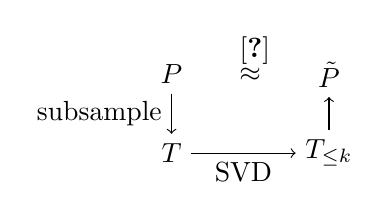
\begin{tikzpicture}[node distance=2.5cm, auto]
    % Nodes
    \node (P) at (0,0) {$P$};
    \node (T) at (0,-1) {$T$};
    \node (Tk) at (2,-1) {$T_{\leq k}$};
    \node (Ptilde) at (2,0) {$\tilde{P}$};

    % Arrows
    \draw[->] (P) to node[left] {subsample} (T);
    \draw[->] (T) to node[below] {SVD} (Tk);
    \draw[->] (Tk) to (Ptilde);

    % Approximate equality
    \node [above] at ($(P)!.5!(Ptilde)$) {\cite{achlioptasFastComputationLowrank2007}};
    \node at ($(P)!.5!(Ptilde)$) {$\approx$};

  \end{tikzpicture}
  \caption{An illustration of the low-rank recommendation algorithm process implied by the Eckart-Young theorem.}
  \end{figure}

  \textbf{Quantum and quantum-inspired-classical recommendation algorithms.} Based on the aforementioned idea, the quantum recommendation algorithm tries to compute and generate the quantum state $|\widetilde{(T_{\le k})_i}\rangle$\footnote{The wavy notation denotes approximation, see section \ref{sec:more_notations}.} then measure it, so as to provide a potentially good recommendation to user $i$. Under the hood, the quantum algorithm extends the quantum phase estimation algorithm\cite{nielsen_chuang_qcqi} to quantum singular value estimation(QSVE), and uses QSVE to project $\ket {T_i}$ onto a subspace spanned by right singular vectors whose corresponding singular values are greater than threshold $\sig$. In the quantum algorithm, $T$ is assumed to take values 0 and 1 only, which naturally results from a "thumb up/down" system and serves as a simplification. We'll inherit and use the binary simplification in our analysis, too.

  \begin{algorithm}[t]
    \caption{Precise Singular Value Projection (Adapted from \cite{q_recommend_sys})}
    \label{algo:q_svd_proj_precise}
    \begin{algorithmic}[1]
      \Require (Preference) matrix $T\in\mathbb R^{m\times n}$; Vector $\v x\in\mathbb{R}^n$ to be projected; Threshold parameter $\s\ge 0$.
      \Ensure $\ket{\v x}$ projected onto $\laspan \{\v v_i|\sig_i\ge\sig\}$, where $\ket{v_i}$ are the left singular vectors of $T$ and $\s_i$ are their corresponding singular values.

      \State Create $\ket\varphi\gets\ket{\v x}$ via the oracle provided by quantum-accessible classical database. Suppose $\ket{\v x}=\sum_{i=1}^n \a_i\ket{\v v_i}$.
      \State Apply (precise) Quantum SVD on $\ket{\v x}$:
        \[\ket \varphi\gets\sum_i\alpha_i\ket{\v v_i}\ket{\sigma_i}\]
      \State Apply \textbf{Quantum If} condition on $\ket{\s_i}$:
        \[\ket \varphi\gets
        \sum_{{\s}_i\ge\s}\alpha_i\ket{\v v_i}\ket{\sigma_i}\ket{1}
        +\sum_{{\s}_i<\s}\alpha_i\ket{\v v_i}\ket{\sigma_i}\ket{0}
        \]
      \State Uncompute $\s_i$:
        \[\ket\varphi\gets
        \sum_{{\s}_i\ge\s}\alpha_i\ket{\v v_i}\ket{1}
        +\sum_{{\s}_i<\s}\alpha_i\ket{\v v_i}\ket{0}
        \]
      \State Measure on the second register. \textbf{If} the outcome is $1$, \textbf{Return} the first register.
      \State \textbf{Else}, goto step 1 and \textbf{repeat}.
    \end{algorithmic}
  \end{algorithm}

  \begin{algorithm}[t]
    \caption{Simplified Model of Quantum Recommendation Algorithm(Adapted from \cite{q_recommend_sys})}
    \label{algo:q_recommend_sys_model}
    \begin{algorithmic}[1]
      \Require Preference database matrix $T\in\mathbb R^{m\times n}$; User $i$ to recommend products.
      \Ensure A product $j$ recommended to user $i$.

      \State $k\gets$ some reasonable rank cutoff parameter that can seperate data from noise.
      \State $\ket\psi\gets\textsc{PreciseSingularValueProjection}(T,T_i,\sigma_k)$.
      \State \textbf{Measure} $\ket\psi$ in the computational basis and get a product $j$.
    \end{algorithmic}
  \end{algorithm}

  Similarly, the quantum-inspired-classical recommendation algorithm \cite{ewin_tang_ciq} generates an approximation to $T_{\le k}$ before sampling to generate recommendations. This algorithm is also based on SVD, but uses a probabilistic downsampling technique developed by Frieze et al. \cite{frieze2004fast} to achieve acceleration over traditional deterministic algorithms. For more details of both algorithms, please refer to appendix \ref{appendix:algo_detail} or the original literature.

  The error analysis of both algorithms are quite complicated. For a clearer presentation, we adopt a reasonably simplified model, where we ignore the error incurred by quantum phase estimation or matrix downsampling, and the singular value threshold $\sig$ is substituted with the number of ranks to be preserved ($\sig\approx\sig_k\to k$). The reason for the first simplification is that errors don't have a big impact on our DP analysis. The second simplification is based on the observation that the cutoff parameter is usually tuned by human operators such that the algorithm can distinguish data from noise. Different forms of parameters would just lead to similar results after manual tuning, so there's no difference between using a threshold and picking the first $k$ terms in an ordered array of singular values. Formally, the simplified model of both algorithms can be defined as follows:

  \begin{definition}[Simplified  Recommendation Algorithms]\label{def:simplified_algo_model}
    \begin{enumerate}
      \item The quantum recommendation algorithm $\A_{\rm RQ}^{k}$ takes in a preference database matrix $T$, a user index $i$, computes $(T_{\le k})_i$ and samples a product $j$ from $(T_{\le k})_i$ by $\ell^2$-norm sampling as its output.
      \item The classical recommendation algorithm $\A_{\rm RC}^{k}$ takes in a preference database matrix $T$, a user index $i$, computes $T_{\le k}$ and samples a product $j$ from $i$-th row of $T_{\le k}$ by $\ell^2$-norm sampling as its output.
    \end{enumerate}

    In both algorithms, $k$ is a rank cutoff parameter (usually tuned and chosen by human operators) such that the algorithm can separate data from noise. By the low-rank assumption, $k$ is in the order of $\rank (P)\sim\polylog(m,n)$, or $k=\O(\polylog(m,n))$.
  \end{definition}

  \subsection{Differential Privacy} Differential privacy (DP) is a framework that seeks to quantify the privacy-preserving ability of (typically randomized) algorithms that take databases as inputs. The basic idea is that when neighbouring databases, denoted as $D$ and $D'$, are provided as inputs, the outputs of a differentially private algorithm should remain close, revealing minimal information about the changes in the database. Databases are usually modeled as a collection of records, and neighbouring databases are those that differ in only one record. Formally, we have the following definition of differential privacy:
  \begin{definition}[Differential Privacy\cite{dwork_algodpbook}]
    A randomized algorithm $\A$ is $(\eps,\delta)$-differentially private if for all neighbouring databases $D$ and $D'$, and for all subset $S\subseteq\image \A$,
    \[
      \Pr\big(\A(D)\in S\big)\le e^\eps\Pr\big(\A(D')\in S\big)+\delta.
    \]
  \end{definition}

  In DP terminology, such randomized algorithms are known as curating mechanisms. Many of these mechanisms simply add noise to the data to obscure them, such as the Laplace mechanism \cite{dwork_algodpbook}.

  \textbf{DP of recommendation problem.} For the recommendation problem, a record is usually a tuple in the form of (user $i$, product $j$, rating $T_{ij}$), corresponding to an entry in the preference database matrix $T$. Thus, in this context, neighbouring databases are preference database matrices $T,T'$ that differ by only one entry. Then our problem is to find DP-parameters $(\eps,\delta)$ such that the following proposition holds:
  \begin{equation}\begin{aligned}
    \Pr\big(\A_{\rm RQ}^k(T,i)=j\big)
    \le
    e^\eps \Pr\big(\A_{\rm RQ}^k(T',i)=j\big) + \delta\\
    \forall\  \text{typical user }i,\forall\  \text{product }j
  \end{aligned}\label{eq:dp_prop}\end{equation}
  for all neighbouring matrices $T$ and $T'$.

  Note that in our context $T$ and $T'$ are binary matrices that differ by only one entry. Suppose $T$ and $T'$ differ at the $(i,j)$-th entry, then the relation between them can be represented as $T'=T\oplus \v e_i \v e_j^\dag$, where $\oplus$ is the addition modulo 2. As a result, $T$ and $T'$ satisfy the conventional definition of neighbouring databases in differential privacy, $||T-T'||_1=|T-T'|_F=1$. In the following analysis, we'll focus on the case where $T'=T+\v e_i \v e_j^\dag$; that is, changing an entry of $T$ from $0$ to $1$. The other side can be analyzed similarly.

  For the quantifier over users, it seems desirable to require $\eqref{eq:dp_prop}$ to hold for all users. However, prior work (Theorem 3.3 of \cite{q_recommend_sys}) has shown that it is infeasible to provide reliably good recommendations for users with very little interaction and preference records. Therefore, we relax this requirement and focus only on \textit{typical users}—those whose number of preference records is close to the average (see section \ref{sec4:dp_res}).

  \textbf{LORA as a curating mechanism.} Many recommendation algorithms are based on extracting the low-rank components of $T$ before sampling a high value entry from it, which we will call the LORA mechanism for short. The LORA  mechanism captures the principal components of a matrix database while filtering out noise; it put users and products into groups, and tends to ignore person-specific behaviours, which are part of personal privacy. Such utility makes these algorithms similar to a privacy curating mechanism; and we'll show later that indeed they are.

  \subsection{More Notations}\label{sec:more_notations}
  As our research topic is multi-disciplinary, notations can be a bit complex sometimes. We seek to clarify some of them in this section.

  \textbf{Dirac Notations.} In quantum computation, it is common to use $\ket v$ to denote a (column) vector $\v v$, and $\bra v$ to denote its conjugate transpose $\v v^\dag$. Then the inner product of $\v u$ and $\v v$ can be written as $\v u\cdot\v v=\langle u|v\rangle$, and the outer product can be written as $\v u\v v^\dag=\ket u\bra v$. This notation is often called Dirac notation.
  %, is preferable in many situations compared to traditional vector notations, and we'll use it sometimes\footnote{Though this may cause confusion against amplitude encoding, it'll be clear which convention is used from the context.}.

  % For traditional linear algebra notation,
  We'll use $V_i$ as the $i$-th row of matrix $V$ and $V_{ij}$ to denote the $i,j$-th entry of $V$. We'll use $\v v_i$ to denote the $i$-th column vector of matrix $V$. Furthermore, we'll use $u_j$ to denote the $i$-th component of vector $\v u$. For $\v v_i$, its $j$-th component will be $v_{ij}$ (note that $v_{ji}=V_{ij}$).
  %When traditional notations are not clear enough,
  We'll sometimes use $\bra i A:= \bra {e_i} A\equiv\v e_i^\dag A$ to denote the $i$-th row of $A$, and $A \ket j\equiv A\v e_j$ to denote the $j$-th column of $A$.

  For the low-rank components of matrix, we'll write $A_{\le k}:=\sum_{i\le k}\sig_i \v u_i \v v_i^\dag$ where $A$ has SVD $A=\sum_i \sig_i \v u_i \v v_i^\dag$. As a slight abuse of notation, we'll also write $A_{\ge \sig}:=\sum_{\sig_i\ge\sig}\sig_i \v u_i \v v_i^\dag$.

  For a quantity $Q$, we usually use $\tilde Q$ to denote an approximation of $Q$(but not always). When quantity $Q_1$ is far bigger(or far less) than $Q_2$, we denote $Q_1\gg Q_2$(or $Q_1\ll Q_2$). For a positive integer $N$, we denote its index set $[N]$ as $[N]:=\{1,2,3,...,N\}$.

\section{Methods}\label{sec3:method}
  \textbf{Problem} Suppose the SVD result of a database matrix $T$ is $T=\sum_\l \sig_\l \v u_\l \v v_\l^\dag$, then what is the SVD of its neighbour $T'=T+ \v e_i\v e_j^\dag$, for a given pair of $(i,j)$? The answer to this question will be pivotal to our analysis over the differential privacy of the concerned algorithms. Unfortunately, SVD is not numerically stable, and it is infeasible to express $\sig_\l',\v u_\l',\v v_\l'$ out of $\sig_\l,\v u_\l,\v v_\l$ in a closed-form manner in general.

  In this section, we introduce our methods gathered from quantum mechanics\cite{zjy_qm_textbook, griffiths_qm_textbook} and random matrix theory\cite{feier_randmat, ai_self_regularization, rand_ev_review, rand_mat_textbook, wishart_rand_mat} to overcome this challenging problem. First (Subsection \ref{sec:justify_pert}), we show that the added term $\v e_i\v e_j^\dag$ is small enough to be viewed as a perturbation. Next (Subsection \ref{sec:lora_pert_form}), we improve the perturbation method used in conventional calculations of quantum mechanics to overcome the unstable nature of SVD. Finally, in Subsection \ref{sec:rand_eigenvec_model} we show and characterize the surprising statistical behaviour of the $U,V$ matrix in SVD of large data matrices, and model them as semi-random matrices, completing the last piece needed to derive our main result.

\subsection{Single Element Shift as a Perturbation}\label{sec:justify_pert}
  In this subsection, we show that the added term $\v e_i\v e_j^\dag$ is actually small enough to be viewed as a perturbation, opening ways to perturbation methods.

  Leveraging results from random matrix theory \cite{feier_randmat}, the following theorem shows that the singular values of random noise is in the order of $\O(\sqrt m)$, and the strength of $\v e_i \v e_j^\dag$ is even less significant than that of random noise.

  \begin{theorem}[Marcenko-Pastur\cite{feier_randmat}, Singular Value Distribution of Noise]
    Suppose $E$ is an  $m\times n$ random matrix representing some noise. That is, each entry of $E$ is a random variable i.i.d. of mean $0$ and variance $1$, with $k$-th moment $\E[E_{ij}^k]<\infty$ not dependent on $n$. Then the singular value distribution of $E$ converges to the following distribution as $m\to\infty$ while keeping $n/m=:\a$ constant:
    \begin{align*}
      p_\a'(x)= \left\{\begin{array}{ll}
        \frac{\sqrt{(\lambda_+-x^2)(x^2-\lambda_-)}}{\pi x} & \sqrt{\lambda_-}\le x\le\sqrt{\lambda_+} \\
        0 & \mathrm{Otherwise}
      \end{array}\right.
    \end{align*}
    where $x$ corresponds to $\sigma(E)/\sqrt{m}$ and $\lambda_{\pm}:=(1\pm\sqrt{\a})^2$.
  \end{theorem}

  %\begin{figure}[t]
  %  \centering
  %  \includegraphics[width=0.8\textwidth]{Marcenko-Pastur_sig.jpg}
  %  \captionsetup{skip=0pt}
  %  \caption{[TODO: rescale it to reflect singular value distribution of $E$.]Singular value distribution of a $m\times n$ random matrix with $m=1001, n=1920$, hence $\a=n/m\approx1.92.$ The random matrix $W$ is generated according to $W=YY^\dag$, $Y=X/\sqrt{m}$, and each entry of $X$ are i.i.d. of mean 0 and variance 1 uniform distrbution. The red line is the modified Marcenko-Pastur distribution $p'_\alpha(x)$.}
  %  \label{fig:Marcenko-Pastur_sig}
  %\end{figure}

  From the above theorem, we can see that the singular values of noise with unit variance is confined to the interval $[\sqrt{m\lambda_-}, \sqrt{m\lambda_+}]=[\sqrt{m}(\sqrt{\a}-1),\sqrt{m}(\sqrt{\a}+1)]$ with high probability. Consequently, the singular values of random noise with intensity $I$ are lower bounded by $\sqrt{m}(\sqrt{\a}-1)I$. Assuming $m$ and $n$ are not too close and $I$ is constant, we have the lower bound $\sqrt{m}(\sqrt{\a}-1)I\sim\mathcal O(\sqrt{m})\gg 1$ where "$\gg$" denotes "much greater than". This establishes the following hierarchy of singular values:
  \begin{equation}
    \{\sig\text{ of data}\}\gg\{\sig\text{ of noise}\}\gg\{\sig\text{ of }\v e_i e_j^\dag(=1)\}.\label{eq:hierachy_of_singval}
  \end{equation}
  This hierarchy reveals that the "strength"(singular value) of the $\v e_i e_j^\dag$ term is even smaller than random noises, which is further much weaker than the strength of data. Therefore, it is reasonable to treat $\v e_i \v e_j^\dag$ as a perturbation.

  \subsection{Low Rank Perturbation Form of SVD}\label{sec:lora_pert_form}

  Perturbation methods are been widely used in quantum mechanics \cite{schrodinger1926quantisierung,zjy_qm_textbook,cohen_qm_textbook,griffiths_qm_textbook}, and is a full-fledged subfield in quantum mechanics.
  However, the traditional form of perturbation\cite{griffiths_qm_textbook,zjy_qm_textbook} is unable to capture the "sharp spike" $\v e_i\v e_j^\dag$ and does not exhibit stable behaviour when applied to SVD. To tackle this problem, we propose a new perturbation form as follows.

  \textbf{Low rank perturbation.} Given that $A\to A'=A+\delta A$ where $\delta A=\v e_i\v e_j^\dag$, we introduce the following matrix perturbation form which is better at capturing the "sharp spike" $\v e_i\v e_j^\dag$:
  \begin{equation}
    A=\sum_\l \sig_\l \v u_\l \v v_\l^\dag \,\,\to\,\, A'\cong\sum_\l \sig_\l (\v u_\l+\alpha_\l \v e_i)(\v v_\l+\beta_\l \v e_j)^\dag
    \label{eq:lora_pert_form}
  \end{equation}
  where $\alpha_\l,\beta_\l\in\mathbb R$ are small perturbation coefficients. For notational convenience, let's suppose $\a_\l,\b_\l$ are in the order of $\lambda$, where $\lambda$ is a real parameter representing some small value. Numerical experiments and subsequent analysis show that $\lambda$ is roughly in the order of $\O(1/m)$, asymptotically small in terms of the database size. To verify the effectiveness of the low rank perturbation form, we've conducted some simple numerical experiments and find that $\sum_\l \sig_\l (\v u_\l+\alpha_\l \v e_i)(\v v_\l+\beta_\l \v e_j)^\dag-\sum_\l\sig_\l\v u_\l\v v_\l^\dag$ is able to capture more than $\%99$ of $\delta A$ on average for realworld data.

  We stress that, although the perturbation form $\eqref{eq:lora_pert_form}$ is designed for capturing single element change, it can be used to capture all one-rank perturbation $\v u\v v^\dag$, by simply replacing $\a_\l\v e_i,\b_\l\v e_j^\dag$ with $\a_\l\v u,\b_\l\v v^\dag$. Furthermore, it can be generalized and applied to few-rank perturbation like $\delta A'=\v u^{(1)}(\v v^{(1)})^\dag+\v u^{(2)}(\v v^{(2)})^\dag+\v u^{(3)}(\v v^{(3)})^\dag+...$ by adding more $\alpha_{\l}^{(2)}\v u^{(2)},\beta_{\l}^{(2)}\v v^{(2)},\alpha_{\l}^{(3)}\v u^{(3)},\beta_{\l}^{(3)}\v v^{(3)},...$ terms, which is specifically useful in data analysis and random matrix theory on low-rank perturbation problems. So we will call it the low-rank perturbation form.

  \subsection{Semi-random Model for SVD of Large Data Matrix}\label{sec:rand_eigenvec_model}

  Suppose $A$ is a large database matrix (e.g. a large recommendation database matrix, or the entire MNIST\cite{mnist} database), and its SVD is $A=\sum_\l\sig_\l\v u_\l\v v_\l^\dag$. At first glance, one would probably think $\v u_\l$ and $\v v_\l$ are vectors representing different preference categories of users and products, thus containing good amount of information and have \textit{high regularity}. But in fact, the value of their components barely exhibit regularity and  behave more like random noise than to structured data. Real-world categories don't tend to be orthogonal to each other; To get orthogonal singular vectors, the SVD algorithm screws up the original categories, resulting in dirty, though orthogonal vectors.

  %Formally, the Johnson-Lindenstrauss lemma states that $\O(e^{\varepsilon N})$ close-to-orthogonal(with $\varepsilon$ error allowed) can be crammed into an $N$-dimensional space. To fill up the $N$-dimensional space, After the cramming process, many vectors appear unrecognizable and appear as if they're drawn from a uniform random distribution over $S^{N-1}$.

  % appear inrecognizable and random

  During the optimization process, more prominent categories are more likely to be preserved, while less prominent categories have to make their way out by being orthogonal to the more prominent ones. Those weaker categorizes may end up being so distorted and messy that they look like random noise. This phenomenon is also supported by the famous Johnson-Lindenstrauss lemma\cite{johnson_lindenstrauss_elem}, which implies that machine learning algorithms(such as PCA and SVD) can cram more information into fewer dimensions by mixing them up.

  To utilize this property and capture the random behaviour, one can model the data matrix as an object whose behaviour is somewhat close to a random matrix.

  In random matrix theory, it has been shown that the normalized eigenvectors of a fully random matrix is usually uniformly distributed on hypersphere $S^{n-1}:=\{\v x\in\mathbb R^n|\,|\v x|^2=1\}$. Intuitive as the result is, it is not trivial to prove it. Formally, we have the following theorem:
  \begin{theorem}[Singular Vector Distribution of Wishart Matrices \cite{wishart_rand_mat}]
      Suppose $A$ is a $m\times n$ random matrix. That is, each entry of $A$ is a random variable i.i.d. of mean $0$ and variance $1$, with $k$-th moment $\E[E_{ij}^k]<\infty$ not dependent on $n$. Then $U$ and $V$ are uniformly distributed on the manifold of unitary matrices equipped with Haar measure. As a result, column and row vectors of $U$ and $V$ are uniformly distributed on $S^{m-1}$ and $S^{n-1}$, respectively.
  \end{theorem}

  This phenomenon, known as \textit{delocalization} \cite{rand_ev_review} in random matrix theory, implies that eigenvector components of random matrices lack strong patterns. In contrast, \textit{localization} occurs when matrix entries are strongly correlated, resulting in eigenvectors with larger, structured components.

  In practice, the preference database matrix $T$ is not a truly random matrix. For realworld cases, there are usually a few strong patterns in database $T$(strong correlation) that can be captured by the leading singular vectors(columns of $U$ and $V$), resulting in localization of vector components and deviation from uniform distribution. Fortunately, \textit{rows} of $U$ and $V$(the same component across different singular vectors) are still very random and barely show any regularity. Moreover, it is very rare to have strong correlations between certain rows of $U$ and $V$.

  Such characteristic of real-world data is confirmed by our numerical experiments, with details recorded as follows:
  \begin{enumerate}
    \item \textbf{When look vertically(columns of $U,V$)}, you find that the leading singular vectors($\v u_1, \v v_1, \v u_2, \v v_2...$) tend to have large and regular component values, while components of later singular vectors($...,\v u_{97}, \v v_{97}, \v u_{98}, \v v_{98},...$) are rather random and faint(small value). That is to say, singular vectors corresponding to larger singular values have higher regularity, and those corresponding to smaller singular values are more similar to random noise.
    \item \textbf{When look horizontally(rows of $U,V$)}, it is even worse — there's no regularity at all. SVD has no reason to preserve regularity among one certain component across different singular vectors; The entries in a row of $U$ or $V$ seem to be just random numbers, with no apparent pattern or correlation.
  \end{enumerate}

  \begin{figure*}[!t]
    \centering
    \includegraphics[scale=0.56]{u_stat_movielen.jpg}
    \includegraphics[scale=0.56]{v_stat_mcimage.jpg}
    \caption{\textbf{Distribution} of components of $U_i$ and $V_j$ on some real-world data. \textbf{Left}: Histogram of $\uli=(U_i)_\l$ of the MovieLens \cite{dataset_movielens} dataset. Due to hardware limitations, dataset is subsampled by a factor of 10 and only the 500 components are computed. \textbf{Right}: Histogram of $\vlj=(V_j)_\l$ of a large matrix converted from a $1001\times 1920$ image(see appendix \ref{appendix:dataset_info} for more details). \textbf{Curves} are corresponding p.d.f. of distribution $S\mathrm{Proj}(m),S\mathrm{Proj}(n)$ respectively. Note that $p_{S\mathrm{Proj}(n)}(\cdot)$ is quite similar to a normal distribution for large $n$. While $u_{\l i}$ and $v_{\l j}$ aren't obeying $S\mathrm{Proj}$ perfectly, the proposed distribution seems to be a good approximation.}
    \label{fig:uv_stat}
  \end{figure*}

  Incorporating the previous insights, we propose the following condition to capture the semi-random behaviour of $U$ and $V$ and the original preference database matrix $T$:

  \begin{definition}[Semi Random Eigenvector Condition]
    A matrix $T$ with SVD $T=U\Sig V^\dag$ satisfies Semi Random Eigenvector Condition(SREC) if
    \begin{enumerate}
      \item $U_i\sim \mathrm{Uniform}(S^{m-1})$ for $1\le i\le m$,
      \item $V_j\sim \mathrm{Uniform}(S^{n-1})$ for $1\le j\le n$, and
      \item For given $1\le i\le m$ and $1\le j\le n$, $U_i$ and $V_j$ are independent.
    \end{enumerate}

    where $S^{N-1}$ denotes the $N-1$-dimensional sphere $S^{N-1}=\{\v x|x_1^2+x_2^2+\cdots+x_N^2=1\}$ and $\mathrm{Uniform}(S^{N-1})$ represents a uniform distribution on $S^{N-1}$.
  \end{definition}

  When we model a matrix under the SREC, our goal is not to claim the preference database matrix is a random matrix; Rather, we aim to show that the portion of input matrices that violates certain properties(such as DP) is asymptotically small(small probability), making it highly unlikely for real-world databases to fall into the bad niche and violate these properties. Furthermore, modelling $U_i$ and $V_j$ as random variables enables a lot of calculations that would be otherwise infeasible due to the complex numerical nature of SVD.

  Finally we show some simple results of a uniform distribution over $S^{N-1}$, which will be useful in our following calculations.

  \begin{theorem}[Properties of $\mathrm{Uniform}(S^{N-1})$]\label{thm:uniform_S}
    Suppose $\v X=(X_1,X_2,...,X_N)$ is a random vector drawn from a uniform distribution on $S^{N-1}$, with $N\ge 2$. Denote $\{1,2,\cdots,N\}$ as $[N]$, then $\v X$ satisfies the following properties:
    \begin{enumerate}
      \item \textbf{(Individual Component Distribution)} For every individual component $X_i$ of $\v X$, $X_i\sim S\text{Proj}(N)$(Sphere Projected), a custom distribution with the following p.d.f:
      \[
        p_{S\text{Proj}}(x;N)=\left\{\begin{array}{ll}
          \frac{\,\,\,\,(1-x^2)^{\frac{N-3}{2}}}{B\big(\frac{1}{2},\frac{N-1}{2}\big)} & x\in[-1,1], \\
          0 & x\notin [-1,1].
        \end{array}\right.
      \]
      Furthermore, $p_{S\text{Proj}}(x;N)$ converges to a normal distribution with mean $0$ and variance $1/N$ as $N\to\infty$.
      \vspace{0.2em}
      \item \textbf{(Individual Component Statistics)} For every individual component $X_i$, $\E[X_i]=0$ and $\Var[X_i]=\E[X_i^2]=\frac 1N$.
      \vspace{0.2em}
      \item \textbf{(Partial Square Norm)} For a subset $I\subseteq[N]$, $|\v X_{\in I}|^2:=\sum_{i\in I}X_i^2\sim \mathrm{Beta}\left(\frac{|I|}{2},\frac{N-|I|}{2}\right)$, where $\mathrm{Beta}(a,b)$ is the Beta distribution with parameter $a,b$. Furthermore, $\E\big[|X_{\in I}|^2\big]=\frac{|I|}{N}$ and $\Var\big[|X_{\in I}|^2\big]=\frac{|I|(N-|I|)}{N^2(N/2+1)}$.
      \vspace{0.3em}
      \item \textbf{(Odd Moment)} $\E[X_i^\nu]=0$ for odd $\nu$ and any $i\in[N]$.
      \vspace{0.1em}
      \item \textbf{(Covariance 1)} $\E\left[\prod_{i\in I} X_i\right]=0$ for a subset $I\subseteq[N]$ of components. As a result, $\mathbf{Cov}[X_i,X_j]=\E[X_iX_j]=0$ for any $1\le i<j\le N$.
      \vspace{0.2em}
      \item \textbf{(Covariance 2)} $\mathbf{Cov}[X_i^2,X_j^2]=-\frac{2}{N^2(N/2+1)}<0$, for $1\le i<j\le N$. Note that $\mathbf{Cov}[X_i^2,X_j^2]=\O(1/N)\cdot \E[X_i^2]\E[X_j^2]$, meaning the correlation is asymptotically small.
    \end{enumerate}
  \end{theorem}

  %\begin{assumption}
  %  Given $i$, $u_{\l i}\iid N(0,\sig_u^2)$ for $\l=1,...,m$; Given $j$, $v_{\l j}\iid N(0,\sig_v^2) $ for $\l=1,...,n$.
  %\end{assumption}

  \begin{table*}[!t]
    \caption{Basic Statistics of Some Commonly Used Recommendation Datasets}
    \centering
    \normalsize
    \begin{tabular}{l|cc|cc}
    \toprule
    Dataset         & $m$  & $n$  & $\eta$ & density $\frac{|T|^2}{mn}$ \\
    \midrule
    Custom Image(appendix \ref{appendix:dataset_info})        & 1001   & 1920   & 441.2  & 0.23           \\
    MovieLens-latest-small\cite{dataset_movielens} & 610  & 9742   & 165.3  & 0.017          \\
    MovieLens-25m\cite{dataset_movielens} & 162541 & 62423  & 153.8  & 0.0027         \\
    Amazon Reviews'23\cite{dataset_amazon}  & 54.51m & 48.19m & 10.49  & 2.2$\times 10^{-7}$  \\
    Google Restaurant\cite{dataset_google_restaurants} & 1.01m  & 65113  & 1.72   & 2.7$\times 10^{-5}$  \\
    \bottomrule
    \end{tabular}
    \label{table:dataset_stats}
  \end{table*}

  %By modeling $\uli$ and $\vlj$ as random variables, we can see that $\delta_{ij}(k)$ is a sum of i.i.d. random variables, forming a random walk. Using the fact that $\v u_\l$ and $\v v_\l$ are normalized vectors and that there components are of normal distribution, we can figure out that  $\sig_u^2=\frac{1}{m}=\E[\uli^2]$, $\sig_v^2=\frac{1}{n}=\E[\vlj^2]$. Then for $k\gg 1$, we should have $\delta_{ij}(k)\approx k\cdot \E[\uli^2+\vlj^2]=k\cdot\left(\frac 1m+\frac 1n\right)$. Define $f(k)=k\cdot\left(\frac 1m+\frac 1n\right)$ and recall that $\delta(k)=\delta_{ij}(k)$, and we would have proved $\textit{1}$ of our core lemma.

\section{Differential Privacy Result}\label{sec4:dp_res}
  In this section, we'll present our main result on the differential privacy properties of the quantum recommendation algorithm. In subsection \ref{sec:typical_user}, we introduce the concept of typical users, which is an important concept for the following analysis; In subsection \ref{sec:main_res}, we present our main result and sketch an outline of its proof; In subsection \ref{sec:core_lemmas}, we prove the necessary lemmas needed for the main result, using the method we've established in the previous section; And finally in subsection \ref{sec:main_res_proof}, we provide a complete proof to our main result.

\subsection{Typical User}\label{sec:typical_user}
  Ideally, the job of a recommendation system is to provide preferred products for \textit{every} user. However, it is unrealistic to provide good recommendations for users who have shown no preference on any product, or to users who barely like any product. To address this issue, a common approach is to focus on \textit{typical} users only(for example, theorem 3.3 in \cite{q_recommend_sys}). We'll also adopt this approach and require the quantum recommendation algorithm to satisfy our main result for typical users only.

  Define average preference record number as $\eta=\frac{\#\text{\normalfont Total Records}}{\#\text{\normalfont Users}}=\frac{|T|^2}{m}.$ Then typical users are defined as users whose preference record number is close to average:

  \begin{definition}[Typical User]
    A user $i$ is called $\gamma$-\textit{typical} if
    $
      \frac{1}{1+\gamma}\le \frac{|T_i|^2}{\eta}\le 1+\gamma
    $
    for some positive parameter $\gamma>0$.
  \end{definition}

  %Then the following theorem guarantees the effectiveness of the quantum recommendation algorithm on \textit{typical users}:
  %\begin{theorem}[Theorem 3.3 from \cite{q_recommend_sys}]
  %  Let $T$ be an $m\times n$ matrix. Let $S\subseteq\{1,2,...,m\}$ be a set of $\gamma$-typical users, with $\gamma$ chosen such that $|S|\ge (1-\zeta)m$ for some $\zeta>0$. Let $\td T$ be an approximation of $T$ such that $|T-\td T|\le\eps|T|$.
    %  Then, there exists a subset $S'\subseteq S$ of size at least $(1-\xi-\zeta)m$ for some $\xi>0$, such that on average over the users in $S'$, the probability that a sample from a row $\td T_i$ is a bad recommendation is
  %  \[
  %    \mathop\mathrm{Prob}_{i\sim U_{S'},j\sim\ell^2(\td T_i)}\big((i,j)\text{\normalfont\, bad}\big)
  %    \le \frac{
  %      \left(\frac{\eps(1+\eps)}{1-\eps}\right)^2
  %    }{
  %      \left(1/\sqrt{1+\gamma}-\eps/\sqrt\xi\right)^2(1-\xi-\zeta)
  %    }
  %  \]
  %  where $U_{S'}$ is the uniform distribution over $S'$.
  %\end{theorem}

  On one hand, the restriction of typical users helps guarantee the effectiveness of the quantum recommendation algorithm(see theorem 3.3 in \cite{q_recommend_sys}. On the other hand, it also bounds $|T_i|^2$ into $[\frac{\eta}{1+\gamma},\ (1+\gamma)\eta]$, which will be a useful yet practical condition in the following analysis. Finally, the following lemma shows that a typical user is still close to typical when database is changed by one record.

  \begin{lemma}\label{lemma:gamma_td}
    Suppose $T'$ is a neighbouring matrix of $T$, then for $\gamma$-typical user $i$, we have
    $
      \frac{1}{1+\td\gamma}\le \frac{|T'_i|^2}{\eta}\le 1+\td\gamma
    $
    given $\frac{\eta}{1+\gamma}>1$. Here, $\td \gamma$ is defined as $\td\gamma = \gamma + \frac{1+\gamma}{\frac{\eta}{1+\gamma}-1}.$
  \end{lemma}

  \noindent\textbf{Proof}
  For any neighbouring matrix $T'$, we have $|T_i|^2-1\le|T'_i|^2\le |T_i|^2+1$. That is to say, we need to find $\td \gamma$ that satisfies
  \[
    \frac{\eta}{1+\td\gamma}\le |T_i|^2-1< |T_i|^2+1\le \eta(1+\td\gamma).
  \]
  By some simple calculation, we find that $\td\gamma=\gamma+\frac{1+\gamma}{\frac{\eta}{1+\gamma}-1}$ is the smallest value satisfying the inequality, given $\sfrac{\eta}{(1+\gamma)}>1$.

\subsection{Main Result}\label{sec:main_res}
  Using previously introduced methods and concepts, we are able to establish the following result, demonstrating that the quantum recommendation algorithm preserves differential privacy under certain conditions.
  \vspace{0.3em}
  \begin{theorem}[Main Result]
    The quantum recommendation algorithm $\A_{\rm RQ}^k$ and quantum-inspired-classical recommendation algorithm $\A_{\rm RC}^k$ satisfies
    \begin{enumerate}
      \item $\left(\frac{1+\td\gamma}{\eta}\frac{k}{n},\,\, \frac{1+\td\gamma}{\eta}\cdot 2.01k\big(\frac 1m+\frac 1n\big)\right)$-DP.
      \item $\left(\td\O\big(\frac 1n\big),\,\, \td\O\big(\frac{1}{\min\{m,n\}}\big)\right)$-DP.
    \end{enumerate}

    for $\gamma-$typical users on SREC input matrices.
  \end{theorem}

  This theorem shows that both recommendation algorithms preserve differential privacy. Additionally, the DP parameters of them decrease as number of products($m$) and users($n$) grow, and are asymptotically small against the numbers, which is a desirable property for DP. More interestingly, the main result shows the quantum recommendation algorithm \textit{naturally} preserves differential privacy even when no extra curating mechanism is added.

  This result is consistent with our everyday experiences. Suppose you're using YouTube or Tiktok, and click into(or like) an video accidentally. Such single incident barely change the recommended content; Users usually have to show preference for multiple similar videos before the recommendation system starts to recommend similar contents for you.

  In the next subsections we focus on the proof of main result; Please refer to the Discussion section \ref{sec5:discuss} for a more detailed discussion on the meaning and implications of our main result.

  \begin{figure}[H]
  \centering
  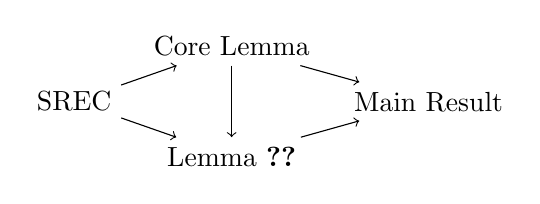
\begin{tikzpicture}[node distance=2.5cm, auto]
    % Nodes
    \node (SREC) at (-2,0) {SREC};
    \node (core_lemma) at (0,0.7) {Core Lemma};
    \node (lemma_2) at (0,-0.7) {\,\,\,Lemma \ref{lemma:row_norm_diff}\,\,\,};
    \node (main_res) at (2.5,0) {Main Result};

    % Arrows
    \draw[->] (SREC) to (core_lemma);
    \draw[->] (SREC) to (lemma_2);
    \draw[->] (core_lemma) to (lemma_2);
    \draw[->] (core_lemma) to (main_res);
    \draw[->] (lemma_2) to (main_res);

  \end{tikzpicture}
  \caption{A diagram illustrating our proof strategy.}
  \end{figure}

  The proof of our main result is a bit winded. To facilitate understanding, here we only sketch an outline of our proof, and postpone the proof with full detail to section \ref{sec:main_res_proof}.
  \vspace{0.3em}

  \noindent \textbf{Outline of Proof} It suffices to show that
  \begin{align}
    \Pr\big(\A_{\rm R}^{k}(T';i)=j\big)
    \le e^\eps \Pr\big(\A_{\rm R}^{k}(T;i)= j\big) + \delta
    \label{eq:line1}
  \end{align}
  holds for the desired values of $\varepsilon, \delta$ for all $\gamma-$typical users on neighbouring databases $T$ and $T'$. Here, $\A_{\rm R}^k$ represents $\A_{\rm RQ}^k$ or $\A_{\rm RC}^k$. Recall that both $\A_{\rm RQ}^{k}$ and $\A_{\rm RC}^{k}$ sample from a row of the low-rank approximation $(T_{\le k})_i$ to provide recommendations to user $i$. That is to say:
  \begin{align}
    \Pr\big(\A_{\rm R}^{k}(T;i)=j\big)=\frac{\big|(T_{\le k})_{ij}\big|^2}{\big|(T_{\le k})_i\big|^2}\label{eq:line2}
  \end{align}
  Plug $\eqref{eq:line2}$ into $\eqref{eq:line1}$, then it expands to
  \begin{align}
    \frac{\big|(T'_{\le k})_{ij}\big|^2}{\big|(T'_{\le k})_i\big|^2}
    \le e^\varepsilon \frac{\big|(T_{\le k})_{ij}\big|^2}{\big|(T_{\le k})_i\big|^2}
    + \delta.\label{eq:line3}
  \end{align}
  Now our task has been reduced to proving $\eqref{eq:line3}$. To prove this inequality, we need to bound the change in the nominator $|(T_{\le k})_{ij}|$ and the denominator $|(T_{\le k})_i|$ for neighbouring matrices $T, T'$. This work is done by the core lemma \ref{lemma:core_lemma} and lemma \ref{lemma:row_norm_diff} respectively, who will be introduced in the next section. Using the lemmas, we're able to show the following relation:
  \begin{gather}
    \frac{\big|(T'_{\le k})_{ij}\big|^2}{\big|(T'_{\le k})_i\big|^2}
    \le \Bigg(1+\frac{k/n}{\big|(T'_{\le k})_{i}\big|^2}\Bigg)
    \cdot\frac{\big|(T_{\le k})_{ij}\big|^2}{\big|(T_{\le k})_i\big|^2}\notag\\
    \qquad\qquad\qquad\quad +\frac{1+\td\gamma}{\eta}\cdot 2.01k\left(\frac1m+\frac 1n\right)\label{eq:line4}
  \end{gather}
  Then the first clause of the theorem immediately follows from $\eqref{eq:line4}$ after some relaxation and bounding. Then we would have proved the first part of the main result.

  Finally, by some order estimation we are able to reduce the first clause into the second clause of the main result, proving that $\mathcal A_{\rm R}^k$ is DP with asymptotically small privacy budget(i.e. DP parameter).
  \hfill\ensuremath{\blacksquare}

\subsection{The Lemmas}\label{sec:core_lemmas}
  In this subsection, we show the lemmas that bound changes between $T_{\le k}$ and $T'_{\le k}$, which are required to prove our main result. In the following expression of probability
  \begin{align*}
    \Pr\big(\A_{\rm R}^{k}(T;i)=j\big)=\frac{\big|(T_{\le k})_{ij}\big|^2}{\big|(T_{\le k})_i\big|^2}=\frac{\big|\langle i|T_{\le k}|j\rangle\big|^2}{\big|\bra{i}T_{\le k}\,\big|^2}
  \end{align*}
  we first characterize the change in the nominator $(T_{\le k})_{ij}$ in Core Lemma \ref{lemma:core_lemma}, then bound the change in denominator $(T_{\le k})_i$ in lemma \ref{lemma:row_norm_diff}.

  Formally, denote $T'_{\le k}-T_{\le k}$ as $\Delta_{\le k}$, and define
  \begin{align}
    \delta(k):=\max_{i'j'}\big|\langle i'|\Delta_{\le k}|j'\rangle\big|,\quad
    \delta_{ij}(k):=\big|\langle i|\Delta_{\le k}|j\rangle\big|,
    \label{eq:delta_def}
  \end{align}
  then we have the following lemma on the maximal difference of matrix entry $\delta(k)$:

  \begin{lemma}[Core Lemma]\label{lemma:core_lemma}
    Suppose $T$ satisfies SREC, and $T'=T+ \delta T=T+ \v e_i\v e_j^\dag$. Define $\delta(k)$ as in $\eqref{eq:delta_def}$ and $f(k)=k\cdot \left(\frac{1}{m}+\frac{1}{n}\right)$. Then for $k\sim \rank\, (T)\ll m,n$ we have:
    \begin{enumerate}
      \item $\delta(k)\approx f(k)$. That is to say, $\delta(k)$ is linear to $k$.
      \item $\Pr\big(|\delta(k)-f(k)|\ge t\Sig\big)\le \frac{1}{t^2}$ for $t> 0$ and sufficiently large $m,n$, where $\Sig=\sqrt{2.01k\cdot\left(\frac 1{m^2}+\frac 1{n^2}\right)}=\O(\sqrt{k})$.
    \end{enumerate}
  \end{lemma}

  \begin{figure*}[!t]
    \centering
    \includegraphics[scale=0.6]{core_lemma_movielen.jpg}
    \includegraphics[scale=0.6]{core_lemma_mcimage.jpg}
    \captionsetup{skip=0pt}
    \caption{Demonstration of the core lemma. $\delta(k)$, $f(k)$ and $95\%$ probability bound by core lemma on some real-world data is computed and plotted. \textbf{Left}: MovieLens \cite{dataset_movielens} dataset. Due to hardware limitations, MovieLens dataset is subsampled by a factor of 10 and only first 500 singular terms are computed. \textbf{Right}: An $1001\times 1920$ image(the same image as in figure \ref{fig:uv_stat}). For small $k$, $\delta(k)$ appears to be linear and close to $f(k)$; For large $k\sim m,n$, $\delta(k)$ saturates to $1$ and grows slower than $f(k)$. Because full-scale SVD is required to do the computation and recommendation databases are typically extremely large and sparse(see table \ref{table:dataset_stats}), we are unable to extend our experiment to larger datasets.}
    \label{fig:main_thm}
  \end{figure*}

  Clause 1 of the above lemma is a basic approximation, while clause 2 gives a more delicate analysis on the probability bounds, providing a with-high-probability result.

  The core lemma demonstrates that the maximal entry change in $\Delta_{\le k}$ is a linear function of $k$, and is far smaller than that of $\Delta:=T'-T$ for practical $k$.
  To understand this, note that $\rank(T)\sim\polylog(m,n)$ is usually far smaller than $m$ and $n$. with a practical rank cutoff $k\sim\rank(T)$, we have $\delta(k)\approx f(k)=\polylog(m,n)\left(\frac{1}{m}+\frac{1}{n}\right)=\tilde O(\frac 1m+\frac 1n)=\td O\big(\frac{1}{\min\{m,n\}}\big)$. Expectation of $\delta(k)$ will then be vanishingly small compared to $m,n$. This result indicates that the low-rank approximation based on SVD curates the change in input quite well.

  To demonstrate and verify the core lemma, we've also conducted numerical experiments on real world data. Given a dataset, $\delta(k)$ is computed for different $k$, and results are shown in figure \ref{fig:main_thm}. The results agree with the core lemma well. Experiments are run on a PC with Intel(R) Core(TM) i7-8750H CPU and 16 GB of memory, and can be done within twenty minutes. Aside from recommendation datasets, we've also conducted experiments on an 2D image, and our theory still works well. Such success suggests that our theory may also be applied to computer vision problems, for example, analyzing the robustness of PCA-based data augmentation techniques\cite{alexnet} under single pixel change.

  \vspace{0.5em}
  \noindent \textbf{Proof of Core Lemma} First of all, we assert\footnote{One can remove this assumption by considering $\delta(k)\cong\delta_{ij}(k)$ as a high probability event(instead of a certain event), that is: $\Pr(\delta(k)=\delta_{ij}(k))=1-o(1).$ Taking this probability into account makes no significant difference in our core lemma, but the analysis will be much more complicated.} that $\delta(k)\approx \delta_{ij}(k)$. $\delta T$ is a perturbation on the $(i,j)$-th entry of $T$, and $\Delta_{\le k}$ should primarily focus on the $(i,j)$-th entry, while other entries are far less affected, suffer only high order corrections. In fact, numerical analysis has also shown that $\delta(k)=\delta_{ij}(k)$ is true for more than $99.5\%$ of the time. Therefore, we can assert that $\delta(k)\approx \delta_{ij}(k)$. In the following proof, we can consider $\delta(k)$ as $\delta_{ij}(k)$, getting rid of the $\max_{ij}$ process.

  \begin{assumption}
    We assume that $\delta(k)=\delta_{ij}(k)$.
  \end{assumption}

  Using the perturbation form introduced in the previous section \ref{sec:lora_pert_form}, we can treat $\delta T=\v e_i\v e_j^\dag$ as a perturbation, and use the low rank perturbation form in the previous section. Suppose SVD of $T$ gives $T=\sum_\l \sig_\l \v u_\l \v v_\l^\dag$, then we have:
  \begin{equation}
    \label{eq:T_pert}
    T'=\sum_\l \sig_\l (\v u_\l+\alpha_\l \v e_i)(\v v_\l+\beta_\l \v e_j)^\dag
  \end{equation}
  where $\alpha_\l,\beta_\l$ are small perturbation coefficients and $\l$ is summed from $1$ to $\min\{m,n\}$. Numerical experiments and subsequent analysis show that, $\a_\l,\b_\l$ is typically in the order of $\O(1/m)$ and $\O(1/n)$, and much smaller than that for small $\l$, making it asymptotically small as $m,n$ grows. $\eqref{eq:T_pert}$ is actually such a good approximation that it captures $\sim 99.9\%$ of $\delta(k)$, as shown in numerical analysis.

  Apply the Eckart-Young theorem to $\eqref{eq:T_pert}$ under constraint $\bra{i}T'\ket{j}=1$, then $\eqref{eq:T_pert}$ can be reduced to an optimization problem after ignoring some higher-order terms(see appendix \ref{append:proof} for detailed derivation). The derived optimization problem is as follows:
  \begin{align*}\begin{split}
    \min_{\td\a_\l,\td\b_\l} \quad &\sum_{\l}\td\a_\l^2+\td\b_\l^2\\
    \text{s.t.}\quad &\sum_\l (\td\a_\l v_{\l j}+\td\b_\l u_{\l i})= 1
  \end{split}\label{eq:opt}\tag{$\star$}\end{align*}
  Using the Cauchy-Schwartz inequality\footnote{Alternatively, Lagrange multiplier method also works.}, we can solve the minimization problem explicitly:
  \begin{gather*}
    \left(\sum_\l \td\a_\l^2+\td\b_\l^2\right)\cdot
    \left(\sum_\l v_{\l j}^2+u_{\l i}^2\right)\qquad\qquad\\
    \qquad\qquad\ge\left(\sum_\l \td\a_\l v_{\l j}+\td\b_\l u_{\l i}\right)^2=1
  \end{gather*}
  We don't care about the actual lower bound of $\sum_\l \td\a_\l^2+\td\b_\l^2$, we care about when the equality holds and the corresponding value of $\a_\l$ and $\b_\l$. Cauchy-Schwartz inequality tells us that the inequality become equality when and only when
  \begin{equation}
    \boxed{\td\a_\l= C\cdot v_{\l j},\quad \td\b_\l= C\cdot u_{\l i}.}
  \end{equation}
  where $C$ stands for a constant. Simple numerical experiments show that $C=1$(and $C=-1$ when $T_{ij}$ shifts from 1 to 0).

  \medskip

  Now we turn back to $\delta(k)$. Recall that $\delta(k)=\delta_{ij}(k)$, and by definition of $\delta_{ij}(k)$ we easily get:
  \begin{align*}
    \delta_{ij}(k)&=\big|\langle i|\Delta_{\le k}|j\rangle\big|
    =\sum_{\l\le k}\sig_\l(\a_\l v_{\l j}+\b_\l u_{\l i}+\a_\l\b_\l)\\
    &=\sum_{\l\le k}\td\a_\l v_{\l j}+\td\b_\l u_{\l i}+\td\a_\l\td\b_\l/\sig_\l\\
    &=\sum_{\l\le k}\vlj^2+\uli^2+\frac{\uli\vlj}{\sig_\l}
  \end{align*}

  Having solved the minimization problem and got the above relation, we are now close to demonstrating the linearity of $\delta(k)$. Note that $\uli$ and $\vlj$ are components of rows $U_i$ and $V_j$, and $U_i$ and $V_j$ are now random vectors under the Semi Random Eigenvector Condition. Using the probabilistic model, we can calculate the expectation and variance of $\delta_{ij}(k)$, and bound it with high probability via Chebyshev's inequality.

  The expectation is simple:
  \begin{align*}
    \E[\delta_{ij}(k)]&=\E\left[\sum_{\l\le k}(v_{\l j}^2+u_{\l i}^2)\right]+\sum_{\l\le k}\frac{\E[\uli]\E[\vlj]}{\sig_\l}\\
    &=k\cdot\left(\frac 1m+\frac 1n\right)+0=f(k)
  \end{align*}

  Thus we have demonstrated the first clause of the lemma $\delta(k)=\delta_{ij}(k)\approx f(k)$, in the sense of expectation value.

  The variance is a bit tricker. Direct computation using theorem \ref{thm:uniform_S} shows that $\mathbf{Cov}[\uli^2+\vlj^2,\uli\vlj]=0$, and
  \begin{gather*}
      \mathbf{Cov}\Big[\uli^2+\vlj^2+\frac{\uli\vlj}{\sig_\l}, u_{pi}^2+v_{pj}^2+\frac{u_{pi}v_{pj}}{\sig_p}\Big]<0\\ \text{for } 1\le \l\neq p\le \min\{m,n\}.
  \end{gather*}

  Then we have the following upper bound for variance of $\delta_{ij}(k)$:
  \begin{gather*}
    \phantom{=}\Var[\delta_{ij}(k)]
    <\sum_{\l\le k}\Var\left[\vlj^2+\uli^2+\frac{\uli\vlj}{\sig_\l}\right]\\
    \le 2\left(\frac{1}{m^2}+\frac{1}{n^2}\right)+\sum_{\l\le k}\Var\left[\frac{\uli\vlj}{\Omega(\sqrt m)}\right]\\
    =2k\left(\frac{1}{m^2}+\frac{1}{n^2}\right)+k\cdot \frac{\O(m^{-1/2})}{mn}
    \le 2.01k\left(\frac{1}{m^2}+\frac{1}{n^2}\right).
  \end{gather*}
  The second inequality follows from the previous estimation that singular value of data is at least in the order of $\O(\sqrt{m})$, no less than singular value of a random noise matrix. As we require $k$ to be the rank cutoff parameter that can distinguish data from noise, we can say that $\sig_k$ should be a singular value of data and thus we have $1/\sig_\l\le1/\sig_k=\O(1/\sqrt{m})$ for $\l\le k$ based on our previous estimation $\eqref{eq:hierachy_of_singval}$. After that, we care about the asymptotic behaviour of $\delta_{ij}(k)$. When $m,n$ are sufficiently large, the second term will be vanishingly small compared to the first term. So we opt to absorb the second into the first term with a slightly increased constant(the last inequality).

  Finally, by Chebychev's inequality, we have the following bound for random variable $\delta(k)=\delta_{ij}(k)$:
  \begin{align*}
    \Pr\left[\Big|\delta(k)-f(k)\Big|\ge t\ \sqrt{2.01k\cdot\left(\frac 1{m^2}+\frac 1{n^2}\right)}\ \right]\le \frac{1}{t^2}
  \end{align*}
  Thus we have proved the second assertion of our core lemma.\qed

  \vspace{.7em}

  In the core lemma, we bounded the change in $(T_{\le k})_{ij}$ between neighbouring database matrices. Next we try to characterize the change in the entire row $|(T_{\le k})_i|$ when $T$ is shifted to $T'$. Similar to core lemma, we have derived the following lemma:
  \begin{lemma}
    \label{lemma:row_norm_diff}
    For $k\ll m,n$, we have
    \begin{enumerate}
    \item $|(\Delta_{\le k})_i |^2=|(T'_{\le k})_i-(T_{\le k})_i\ |^2\approx \frac{k}{n}$,
    \item $|(\Delta_{\le k})_i |^2=|(T'_{\le k})_i-(T_{\le k})_i\ |^2\le 2$.
    \end{enumerate}
  \end{lemma}

  \noindent \textbf{Proof} By low rank perturbation form, we have $\Delta_{\le k}=\sum_{\l \le k}\sig_\l(\a_\l\v e_i\v v_\l^\dag+\b_\l\v u_\l\v e_j^\dag+\a_\l\b_\l\v e_i\v e_j^\dag)\approx \sum_{\l\le k}\td\a_\l\v e_i\v v_\l^\dag+\td\b_\l\v u_\l\v e_j^\dag$. Then we have:
  \begin{align*}
    |(\Delta_{\le k})_i|^2&\cong\left|\v e_i^\dag\sum_{\l\le k}\td\a_\l\v e_i\v v_\l^\dag+\td\b_\l\v u_\l\v e_j^\dag\right|^2\\
    &=\left|\sum_{\l\le k}\td\a_\l\v v_\l+\td\b_\l u_{\l i}\v e_j^\dag\right|^2\\
    &\le\left|\sum_{\l\le k}\td\a_\l\v v_\l\right|^2+\left|\sum_{\l\le k}\td\b_\l u_{\l i}\v e_j^\dag\right|^2\\
    &=\sum_{\l\le k}\td\a_\l^2+\sum_{\l\le k}(\td\b_\l\uli)^2
    =\sum_{\l\le k}\vlj^2+\uli^4
  \end{align*}

  For approximation, we get the following result assuming $m^2\ll n$  ($m^2\sim n$ or $m^2\gg n$ is very rare in real-world databases; see table \ref{table:dataset_stats}):
  \[
    \sum_{\l\le k}\vlj^2+\uli^4= \sum_{\l\le k}\big(\vlj^2+\O(\sfrac 1{m^2})\big)
    \approx \frac kn
  \]

  And for an upper bound, we have:
  \begin{equation}
    \sum_{\l\le k}\vlj^2+\uli^4 \le \sum_{\l\le k}\vlj^2+\uli^2\le 2. \tag*{$\square$}
  \end{equation}

\subsection{Proof of Main Result}\label{sec:main_res_proof}
  Based previous theories and lemmas, we are now ready to give a complete proof on our main result.
  \vspace{0.3em}

  \noindent\textbf{Proof of Main Result}
  We need to prove that
  \begin{align}
    \Pr\big(\A_{\rm R}^{k}(T';i')=j'\big)
    \le e^\eps \Pr\big(\A_{\rm R}^{k}(T;i')= j'\big) + \delta
    \label{eq:line11}
  \end{align}
  holds for the desired values of $\varepsilon, \delta$ for all $\gamma-$typical users $i'$ on neighbouring databases $T$ and $T'=T+\v e_i\v e_j^\dag$. Here, $\A_{\rm R}^k$ represents $\A_{\rm RQ}^k$ or $\A_{\rm RC}^k$.

  Recall that both $\A_{\rm RQ}^{k}$ and $\A_{\rm RC}^{k}$ sample from a row of the low-rank approximation $(T_{\le k})_i$ to provide recommendations to user $i$, then the probability naturally expand to
  \begin{equation}
    \frac{\big|(T'_{\le k})_{i'j'}\big|^2}{\big|(T'_{\le k})_{i'}\big|^2}\le e^\eps \frac{\big|(T_{\le k})_{i'j'}\big|^2}{\big|(T_{\le k})_{i'}\big|^2} + \delta.\label{eq:line12}
  \end{equation}

  As $\delta T=\v e_i\v e_j^\dag$ is a perturbation on the $(i,j)$-th entry of $T$, the change of $T_{\le k}$ should also concentrate on the $i$-th row, especially on the $(i,j)$-th entry. At the meantime, other rows and entries are far less affected, suffer changes of higher orders only. Thus, $\eqref{eq:line12}$ is closest and tightest when $i=i'$ and $j=j'$. Consequently, it suffices to prove the inequality when $(i,j)=(i',j')$ and we'll focus on that case in our subsequent proof. Substituting $i'$ and $j'$ with $i$ and $j$, $\eqref{eq:line12}$ is simplified to the following form:

  \begin{equation}
    \frac{\big|(T'_{\le k})_{ij}\big|^2}{\big|(T'_{\le k})_{i}\big|^2}\le e^\eps \frac{\big|(T_{\le k})_{ij}\big|^2}{\big|(T_{\le k})_{i}\big|^2} + \delta.\notag
  \end{equation}

  For the sake of simplicity, we'll further abbreviate the low-rank approximation $T_{\le k}$ and $T'_{\le k}$ as $\td T$ and $\td T'$ in the proof below. Then we have:
  \begin{align}
    &\phantom{==}\Pr\big(\A_{\rm R}^{k}(T';i)=j\big)
    = \frac{|\td T'_{ij}|^2}{|\td T'_i|^2}\notag\\
    &= \frac{|\td T_{ij}|^2}{|\td T_i|^2} \cdot \frac{|\td T_i|^2}{|\td T'_i|^2} + \frac{|\td T'_{ij}|^2-|\td T_{ij}|^2}{|\td T'_i|^2}\notag\\
    &= \Pr\big(\A_{\rm R}^{k}(T;i)=j\big) \cdot \frac{|\td T_i|^2}{|\td T'_i|^2} + \frac{|\td T'_{ij}|^2-|\td T_{ij}|^2}{|\td T'_i|^2}
    \label{eq:dp_prim_ineq}
  \end{align}
  By lemma \ref{lemma:row_norm_diff}, we have $|\td T_{i}|^2-k/n\le |\td T'_{i}|^2\le|\td T_{i}|^2+k/n$. Then we have the following bound for the multiplicative term $\frac{|\td T_i|^2}{|\td T'_i|^2}$:
  \begin{align*}
    \ln \frac{|\td T_i|^2}{|\td T'_i|^2}
    \le \ln\frac{|\td T'_i|^2+k/n}{|\td T'_i|^2}
    \le \frac{k/n}{|\td T'_i|^2}\le \frac{1+\td\gamma}{\eta}\frac kn
  \end{align*}

  On the other side, we have the following bound for the additive term using the core lemma:
  \begin{align*}
    \frac{|\td T'_{ij}|^2-|\td T_{ij}|^2}{|\td T'_i|^2}
    =\frac{\big(|\td T_{ij}|+|\td T'_{ij}|\big)\big(|\td T_{ij}|-|\td T'_{ij}|\big)}{|\td T_i|^2}\\
    \le \frac{2.01\delta(k)}{{|\td T_i|^2}}\le\frac{1+\td\gamma}{\eta}\cdot 2k\left(\frac 1m+\frac 1n\right)
  \end{align*}
  Plug the two bounds back to the inequality $\eqref{eq:dp_prim_ineq}$, and we would have proved the first statement of the main result theorem.

  Next we proceed to the second statement. For practical recommendation algorithms based on low rank approximation, $k$ is usually taken around $\rank(T)=\polylog(m,n)$. We then estimate the asymptotic behaviour of $\eta$. At first glance, it seems tempting to estimate $\eta\sim |T_i|^2$ as $\O(n)$, proportional to the length of a row; But one might argue that an average user's time is limited and can't spend as much time on rating products as the number of products grow indefinitely. Consequently, we adopt a conservative estimate: $\eta=\Omega(1)$, a constant bigger than $1$, but not increasing asymptotically as $n$ grows. Then we have:
  \begin{align*}
    \A_{\rm R}^{k}&\vDash \mathbf{DP}\left(\frac{1+\td\gamma}{\eta}\frac{k}{n}, \frac{1+\td\gamma}{\eta}\cdot 2k\Big(\frac 1m+\frac 1n\Big)\right)\\
    &=\mathbf{DP}\left(\O\Big(\frac kn\Big),\O\Big(\frac k{\min\{m,n\}}\Big)\right)\\
    &=\mathbf{DP}\left(\td\O\Big(\frac 1n\Big),\td\O\Big(\frac 1{\min\{m,n\}}\Big)\right)
  \end{align*}
  Here "$\vDash$" means "satisfies", and $\A\vDash \mathbf{DP}(\eps,\delta)$ means $\A$ preserves $(\eps,\delta)$-DP. Thus we have proved the main result.\qed

  \begin{figure*}[!t]
    \centering

    \includegraphics[scale=0.56]{unstable_glob_Fnorm_movielen.jpg}
    \includegraphics[scale=0.56]{unstable_glob_Fnorm_mcimage.jpg}
    \captionsetup{skip=0pt}

    \caption{\textit{Global} norm change of classical algorithm output ($|\Delta_{\le k}|$, {\color{violet}purple}) and quantum algorithm output ($\big|(\Delta_{ \le k})_i\,\big|=\Big|\ket{(T'_{\le k})_i}-\ket{(T_{\le k})_i}\Big|$ on different data, {\color{orange}orange}) when changing one element in database, as a function of $k$. $\delta(k)$ is also plotted as a reference. The classical curve({\color{violet}purple}) exhibits unstable behaviour, has higher value and is hard to bound compared to the quantum curve({\color{orange}orange}). \textbf{Left}: MovieLens dataset \cite{dataset_movielens}; \textbf{Right}: An $1001\times 1920$ image (the same image as in figure  \ref{fig:main_thm}).}

    \label{fig:unstable_glob_norm}
  \end{figure*}

\section{Discussion}\label{sec5:discuss}

\subsection{Passive and Asymptotic Differential Privacy}
  Based on our main result \ref{fig:main_thm}, first we note that the quantum recommendation algorithm, or the LORA mechanism, requires no additional noise. Most conventional data curating mechanisms discussed in the DP literatures requiring injecting noise into the data to obscure it before release. Surprisingly, the quantum recommendation algorithm, or the underlying LORA mechanism, is a curating mechanism \textit{on its own}: privacy protection is just a side effect of its intrinsic computation; no extra noise is needed. We call such mechanisms \textit{passive}. This behaviour means the quantum and quantum-inspired-classical recommendation algorithms are \textit{zero computational overhead} curating mechanisms. More interestingly, this intrinsic curating ability is made possible by the probabilistic nature of quantum algorithms. We believe that more quantum algorithms with this property will emerge.

  Moreover, we see that the DP parameters of the quantum recommendation algorithm are \textit{asymptotically small} with respect to database sizes $m,n$, based on our main result \ref{fig:main_thm}. This is in contrast with conventional DP mechanisms(such as Laplace mechanism), whose DP parameters are usually fixed and independent of database sizes. For example, the Laplace mechanism relies on noise calibrated to the query function sensitivity to provide a curating mechanism with desired(but fixed) privacy preserving ability.

  \subsection{Comparison of the Quantum and the Classical Algorithm}
  % 由于figure*会把图片浮动体放到下一页的头部,因此在这里放浮动体的话,就会新开一页,
  % which is NOT wanted. 因此我把图片浮动体的latex放到更前面一些。
  %\begin{figure*}[!t]
  %  \centering

  %  \includegraphics[scale=0.6]{unstable_glob_Fnorm_movielen.jpg}
  %  \includegraphics[scale=0.6]{unstable_glob_Fnorm_mcimage.jpg}
  %  \captionsetup{skip=0pt}

  %  \caption{...}

  %  \label{fig:unstable_glob_norm}
  %\end{figure*}
  Given that the quantum algorithm no longer offers an exponential speedup over the quantum-inspired-classical algorithm, a natural question is: does the quantum algorithm still hold any advantages over the classical counterparts, and what are the differences between them?

  In this section, we conduct a more detailed comparison between the quantum and quantum-inspired-classical recommendation algorithms in terms of their time complexity and privacy preserving ability. We conclude that the quantum algorithm still maintains a significant polynomial advantage in time complexity and also has better privacy protecting potentials.

  \textbf{Computational complexities.} Although the quantum recommendation algorithm has no exponential speedup over the quantum-inspired-classical algorithm, it still provides considerable polynomial speedup over any classical algorithms. Due to the limitation of space, we won't review the quantum-inspired-classical algorithm in full length, and readers can refer to appendix \ref{appendix:algo_detail} for details.

  According to theorem 5.4 in \cite{q_recommend_sys}, the time complexity of the quantum recommendation algorithm is $\td\O\big(\polylog(mn)\cdot\frac{|T|}{\sig_k}\big)$ for most typical users, where $\sig_k$ is the singular value threshold and $\td\O$ hides the log factors incurred by amplifying the failure probability. Based on identity $|T|^2=\sum_i \sig_i^2$, it can be estimated that $\sig_k$ should be in order of $\frac{|T|}{\sqrt k}$. Then the time complexity of the quantum recommendation algorithm can be simply expressed as $\td\O(\sqrt k\cdot \polylog(mn))$.

  The time complexity of the quantum-inspired-classical algorithm is $\td\O\left(\log(mn)\cdot\frac{|T|^{24}}{\sig_k^{24}}\right)$, where $\td\O$ hides the same log factors and some error parameters are hidden for clarity. Using the same techniques, we get a time complexity $\td\O(k^{12}\cdot\log(mn))$.

  Clearly, the quantum algorithm has a significant advantage in the exponent of $k$($\sim$ the exponent of $\rank(T)$) in the time complexity. On the other hand, the exponent of $\log(mn)$ for the quantum algorithm depends on the implementation of quantum RAM\cite{qram} and remains unclear for the time being, so a completely rigorous comparison is not yet possible.

  \textbf{Privacy preserving ability.}
  Next we will give a more detailed comparison on privacy preserving properties between the quantum and quantum-inspired-classical algorithm. Since both algorithms are based on the same low-rank matrix reconstruction technique, they have similar DP parameters and both satisfy $\left(\td\O\big(\frac 1n\big),\td\O\big(\frac 1{\min\{m,n\}}\big)\right)$-DP, as suggested by our main result. However, besides the the DP parameters in common, there're also several subtle differences between them. The quantum algorithm only generates the row $(T_{\le k})_i$ corresponding to the user to be served, whereas the classical algorithm attempts to reconstruct the entire low-rank matrix component $T_{\le k}$. At first glance, this behaviour makes the quantum algorithm less powerful, but $(T_{\le k})_i$ actually enjoys better mathematical properties and contains less information, making the quantum algorithm superior in privacy preserving.

  %actually more numerical stable and leak less privacy, making the quantum algorithm superior in privacy preserving.

  %it actually results in better privacy preserving properties in a surprising way, described as follows.

  %First, the quantum algorithm has better \textit{global} privacy-preserving property.

  %The former contains the change in the entire row of $T\lek$ and corresponds to the output of quantum matrix reconstruction routine, while the latter contains the change in the entire matrix $T\lek$ and reflects the privacy preserving ability of the classical routine.
  %The former contains the change in the entire row $(T\lek)_i$ and the latter contains the change of the entire matrix $T\lek$.

  To see this, let's examine $|(\Delta\lek)_i|$ and $|\Delta\lek|$, which represent the total change in $(T_{\le k})_i$  and $T_{\le k}$ , respectively, when a single entry of $T$ is flipped.  Note that both quantities are 0 when $k=0$ and reach 1 when all ranks are included ($k=\min\{m,n\}$), so it is meaningful to compare them. When we examine $|(\Delta\lek)_i |$, we find it has a good bound and behaves as a relatively smooth function of $k$ (see lemma \ref{lemma:row_norm_diff}). In contrast,  $|\Delta\lek|$ is highly numerical unstable, and has no reasonable bound (see figure \ref{fig:unstable_glob_norm} for numerical experiment results). As a conclusion, from an aggregative perspective, the output of the quantum algorithm leaks less information in $\ket{(T_{\le k})_i}$ in a smooth and controllable manner, whereas the classical algorithm leaks more information in $T\lek$ in an unstable and less predictable way.

  Moreover, the privacy preserving ability of the quantum algorithm is guaranteed by the fundamental quantum theory. \textbf{The fundamental principles of quantum mechanics} guarantee that the quantum state $\ket{(T\lek)_i}$ will be destroyed immediately after measurement, and it is impossible to copy the information contained in the quantum state due to the No-Cloning theorem\cite{nielsen_chuang_qcqi}. On the contrary, the classical algorithm requires additional sampling process, and the system may be susceptible to extra security risks. Information may be leaked before sampling is done via vulnerabilities in software and other parts of the recommendation system. The privacy protection ability of quantum algorithms is guaranteed, in a way similar how the confidential advantage of quantum cryptography and quantum communications is guaranteed by the fundamental law of quantum mechanics.

\subsection{Potential for Extending DP to All Users}
  Our analysis has shown that the quantum recommendation algorithm preserves differential privacy for typical users. However, one might want to extend the privacy guarantee to all users. Next, we propose a possible approach to extend our work and provide privacy guarantee for all users.

  Consider a mechanism constructed as follows. Before the recommendation database is accessed by the vanilla quantum(or quantum-inspired) algorithm, noises are introduced to rows corresponding to non-typical users. Random records are added to (or dropped from) non-typical users till they have enough(or few enough) records to be typical users for a desired $\gamma$ value. The modified matrix $T_{\rm noisy}$ is then used as input to the quantum(or quantum-inspired) recommendation algorithm. As all users \textit{appear} as typical users in the noisy matrix, they all enjoy the same privacy guarantee, as established by our previous analysis. In contrast with bare quantum recommendation algorithm, this probabilistic procedure requires additional noise and is thus active, but it provides privacy guarantee for all users.

  However, proving the effectiveness and correctness of this modified quantum recommendation algorithm is not as straightforward as it might seem, and we haven't address this issue yet. We plan to explore it further in our future research.

\subsection{Limitations}\label{sec:limitations}
  Our study has shown positive results for the quantum and quantum-inspired-classical recommendation algorithm in terms of differential privacy. However, due to the complicated numerical nature of SVD, many restrictions and approximations have to be made before we can reach any meaningful results, posing limitations to our work.


% \begin{figure*}[!t]
% \centering
% \subfloat[Case I]{\includegraphics[width=2.5in]{img2_bin.jpg}%
% \label{fig_first_case}}
% \hfil
% \subfloat[Case II]{\includegraphics[width=2.5in]{img2_bin.jpg}%
% \label{fig_second_case}}
% \caption{Simulation results for the network.}
% \label{fig_sim}
% \end{figure*}

% An example of a floating table. Note that, for IEEE style tables, the
% \caption command should come BEFORE the table and, given that table
% captions serve much like titles, are usually capitalized except for words
% such as a, an, and, as, at, but, by, for, in, nor, of, on, or, the, to
% and up, which are usually not capitalized unless they are the first or
% last word of the caption. Table text will default to \footnotesize as
% the IEEE normally uses this smaller font for tables.
% The \label must come after \caption as always.
%
%\begin{table}[!t]
%% increase table row spacing, adjust to taste
%\renewcommand{\arraystretch}{1.3}
% if using array.sty, it might be a good idea to tweak the value of
% \extrarowheight as needed to properly center the text within the cells
%\caption{An Example of a Table}
%\label{table_example}
%\centering
%% Some packages, such as MDW tools, offer better commands for making tables
%% than the plain LaTeX2e tabular which is used here.
%\begin{tabular}{|c||c|}
%\hline
%One & Two\\
%\hline
%Three & Four\\
%\hline
%\end{tabular}
%\end{table}


% Note that the IEEE does not put floats in the very first column
% - or typically anywhere on the first page for that matter. Also,
% in-text middle ("here") positioning is typically not used, but it
% is allowed and encouraged for Computer Society conferences (but
% not Computer Society journals). Most IEEE journals/conferences use
% top floats exclusively.
% Note that, LaTeX2e, unlike IEEE journals/conferences, places
% footnotes above bottom floats. This can be corrected via the
% \fnbelowfloat command of the stfloats package.

\section{Conclusion}
  Using perturbation methods and random matrix theory, we analyzed the differential privacy properties of the quantum recommendation algorithm\cite{q_recommend_sys} $\mathcal{A}_{\rm RQ}^k$ and the quantum-inspired-classical recommendation algorithm\cite{ewin_tang_ciq}$\mathcal{A}_{\rm RC}^k$. Our calculation reveals that both algorithms preserve $\big(\td\O\big(\frac 1n\big),\,\, \td\O\big(\frac{1}{\min\{m,n\}}\big)\big)$-DP under reasonable restrictions without any external noise. Nevertheless, a more detailed comparison shows that the quantum algorithm has better privacy preserving potential than the classical algorithm.

  During our analysis, we proposed a novel perturbation method tailored for low-rank perturbation and modelled the outcome of SVD as semi-random matrices, addressing the challenging SVD-perturbation problem. To verify our assumptions and results, we conducted numerical experiment on real-world data are conducted, and and the results are supportive to our theory.

% conference papers do not normally have an appendix

% use section* for acknowledgment
\ifCLASSOPTIONcompsoc
  % The Computer Society usually uses the plural form
  \section*{Acknowledgments}
\else
  % regular IEEE prefers the singular form
  \section*{Acknowledgment}
\fi

% Anonymous ver.
%The authors are grateful to XXX, who helped us rule out the infeasible path of seeking an explicit solution to the SVD perturbation problem. We would like to thank XXX for guiding us into the field of random matrix theory. We also thank XXX for insightful discussions on the sampling process of $U_i$, which later guided us toward powerful high-dimensional probability theories. We are also grateful to XXX for providing us with some key references, which helped us find the information on the distribution of eigenvectors in random matrices.

The authors are grateful to Ke'an Chen, who helped us rule out the infeasible path of seeking an explicit solution to the SVD perturbation problem. We would like to thank Qi Zhou for guiding us into the field of random matrix theory. We also thank Chun'an Shi for insightful discussions on the sampling process of $U_i$, which later guided us toward powerful high-dimensional probability theories. We are also grateful to Chengye Li for providing us with some key references, which helped us find the information on the distribution of eigenvectors in random matrices.

\newpage

% references section

\bibliographystyle{IEEEtran}
\bibliography{libpaper}

%\newpage

\appendix

\subsection{Deferred Derivations and Proofs}\label{append:proof}

\subsubsection{Reducing $\eqref{eq:T_pert}$ to $\eqref{eq:opt}$}
  Recall what we have is:
  \begin{align*}
    \left\{\begin{array}{l}
      \bra i T\ket j=0,\,\,\bra i T'\ket j=1 \\
      T=\sum_\l \sig_\l\v u_\l\v v_\l^\dag \\
      T'=\sum_\l \sig_\l (\v u_\l+\alpha_\l \v e_i)(\v v_\l+\beta_\l \v e_j)^\dag
    \end{array}\right.
  \end{align*}

  Define $\Delta=T'-T$ and examine its $(i,j)$-th entry, we acquire the following constraint:
  \begin{align*}
    \bra{i}\Delta\ket{j}=1\ \Rightarrow
    \sum_\l \sig_\l(\a_\l v_{\l j}+\b_\l u_{\l i}+\a_\l\b_\l)=1
  \end{align*}
  where $v_{\l j}$ stands for the $j$-th component of $\v v_\l$, and $u_{\l i}$ stands for the $i$-th component of $\v u_\l$.\footnote{Note that $u_{\l i}=U_{i\l}$ and $v_{\l j}=V_{j\l}$ — the order of subscripts are reversed compared to ordinary matrix notation.}. Recall that $\a_\l,\b_\l$ are small perturbation coefficients, so the last term $\a_\l\b_\l$ can be ignored as they are of higher order compared to $\a_\l v_{\l j}+\b_\l u_{\l i}$. Then we have
  \begin{align}
    &\sum_\l \sig_\l(\a_\l v_{\l j}+\b_\l u_{\l i}+\a_\l\b_\l)\nonumber\\
    =&\sum_\l \sig_\l(\a_\l v_{\l j}+\b_\l u_{\l i}+\O(\lambda^2))\nonumber\\
    \cong &\sum_\l \sig_\l(\a_\l v_{\l j}+\b_\l u_{\l i})\nonumber\\
    \implies &\sum_\l \sig_\l(\a_\l v_{\l j}+\b_\l u_{\l i})\cong 1
    \label{eq:constraint_1}
  \end{align}

  % 老版本文本
  %On the other hand, while $k<\min\{m,n\}$, $T'_{\le k}$ tries to approximate $T'$ as much as possible under the low rank constraint. That is to say, $\a_\l,\b_\l$ should be chosen to minimize the following remnant error:

  On the other hand, while $k<\min\{m,n\}$, the Eckart-Young theorem tells us that $T'_{\le k}$ is the closest matrix to $T$ among all $\rank\le k$ matrices. That is to say, $\a_\l,\b_\l$ should be chosen to minimize the following remnant error to approach the true $T_{\le k}'$:
  \begin{align*}
    &\phantom{=}\a_\l,\b_\l
    =\argmin_{\a_\l,\b_\l}\left|T'_{\le k}-T'\right|=\argmin_{\a_\l,\b_\l}\left|T'_{\le k}-T'\right|^2\\
    &=\argmin_{\a_\l,\b_\l}\Bigg|\sum_{\l\le k}\sig_\l(\v u_\l+\a_\l\v e_i^\dag)(\v v_\l+\b_\l\v e_j)^\dag \\
    &\qquad\qquad\qquad\qquad\qquad-\sum_\l\sig_\l\v u_\l\v v_\l^\dag-\v e_i\v e_j^\dag\Bigg|^2\\
    &=\argmin_{\a_\l,\b_\l}\Bigg|
      \sum_{\l\le k}\sig_\l\Big(\a_\l\v e_i\v v_\l^\dag+\b_\l\v u_\l\v e_j^\dag\Big)\\
      &\qquad\qquad\qquad\qquad\qquad+
      \Bigg(\sum_{\l\le k}\sig_\l\a_\l\b_\l-1\Bigg)\v e_i\v e_j^\dag
    \Bigg|^2
  \end{align*}

  This is effectively turning the complicated optimization process over \textit{matrices} $T'_{\le k}$ with constraint $\rank(T'_{\le k})\le k$ into a simple optimization process over \textit{real numbers} $\a_\l,\b_\l$, greatly simplifying the mathematics. This is similar to some variational methods, such as Ritz's variational method\cite{ritz_method} and Variational Quantum Eigensolver(VQE)\cite{vqe}.

  Now we examine the two summations terms in the last line. The second summation term is of higher order compared to the first summation, so we can ignore it. So our minimization problem would primarily focus on the first summation, which serves as the first order correction of the perturbation.

  For the first summation, using identity
  \[
    |\v u_1\v v_1^\dag+\v u_2\v v_2^\dag|^2=|\v u_1\v v_1^\dag|^2 + |\v u_2\v v_2^\dag|^2 + 2\cdot\langle{\v u_1}|{\v u_2}\rangle\langle{\v v_1}|{\v v_2}\rangle,
  \]
  we see that squared norm of orthogonal outer products are separable. So we can separate the $\v e_i\v v_\l^\dag$ and $\v u_\l\v e_j^\dag$ terms of different $\l$, as $\v u_\l$ and $\v v_\l$ are orthogonal to each other.

  Separating between $\v e_i\v v_\l^\dag$ and $\v u_\l\v e_j^\dag$ is a bit trickier, as they aren't completely orthogonal. Fortunately, they \textit{overlap very little}, meaning that they're approximately orthogonal. To see this, recall that $\v u_\l$ is the $\l$-th left singular vector of $T$, indicating that $|\v u_\l|=1$. On the other hand, all its "strength" is spread out across $m$ components. Suppose $m$ is very large, then $u_{\l i}\sim \O(1/m)$ should be quite small on average. Then we have:
  \[
    \langle \v e_i|\v u_\l\rangle=u_{\l i}\sim \O(1/\sqrt{m}),\quad \langle \v v_\l|\v e_j\rangle=v_{\l j}\sim \O(1/{n})
  \]
  Using the same relation again, we can ignore the overlap between $\v e_i\v v_\l^\dag$ and $\v u_\l\v e_j^\dag$, and provide a good approximation:
  \begin{align*}
    |\v e_i\v v_\l^\dag+\v u_\l\v e_j^\dag|^2&=|\v e_i\v v_\l^\dag|^2 + |\v u_\l\v e_j^\dag|^2 + 2\cdot\langle\v e_i|\v u_\l\rangle\langle\v v_\l|\v e_j\rangle\\
  &=|\v e_i\v v_\l^\dag|^2 + |\v u_\l\v e_j^\dag|^2 + \O(\sfrac1{\sqrt{mn}})\\
    &\cong |\v e_i\v v_\l^\dag|^2 + |\v u_\l\v e_j^\dag|^2
  \end{align*}

  Back to the minimization problem, now we can continue:
  \begin{align*}
    &=\argmin_{\a_\l,\b_\l}\left|
      \sum_{\l\le k}\sig_\l\Big(\a_\l\v e_i\v v_\l^\dag+\b_\l\v u_\l\v e_j^\dag\Big)+
      \Bigg(\sum_{\l\le k}\sig_\l\a_\l\b_\l-1\Bigg)\v e_i\v e_j^\dag
    \right|^2\\
    &= \argmin_{\a_\l,\b_\l}\left|\sum_{\l\le k}\sig_\l\Big(\a_\l\v e_i\v v_\l^\dag+\b_\l\v u_\l\v e_j^\dag\Big)\right|^2+\O(\lambda^4)\\
    &= \argmin_{\a_\l,\b_\l}\sum_{\l\le k}(\sig_\l\a_\l)^2|\v e_i\v v_\l^\dag|^2 + \sum_{\l\le k}(\sig_\l\b_\l)^2|\v u_\l\v e_j^\dag|^2\\
    &\qquad\qquad\qquad\qquad\qquad\qquad+\O\Big(\frac{\lambda^2}{\sqrt{mn}}\Big)+\O(\lambda^4)\\
    &= \argmin_{\a_\l,\b_\l}\sum_{\l\le k}(\sig_\l\a_\l)^2+(\sig_\l\b_\l)^2+\O\Big(\frac{\lambda^2}{\sqrt{mn}}\Big)+\O(\lambda^4)\\
    &\cong \argmin_{\a_\l,\b_\l}\sum_{\l\le k}(\sig_\l\a_\l)^2+(\sig_\l\b_\l)^2.
  \end{align*}
  In the final step, we have thrown terms of higher orders. Note that for large $k$, $\sig_\l$ decreases and the thrown terms becomes relatively big, then the approximation gradually breaks, resulting in the "$k\ll m,n$" condition in the core lemma. Take $k=\min\{m,n\}$, and put the above equation together with $\eqref{eq:constraint_1}$, then we have the following constraint optimization problem for determining $\a_\l$ and $\b_\l$:
  \begin{align*}
    \min_{\a_\l,\b_\l}\quad &\sum_{\l}(\sig_\l\a_\l)^2+(\sig_\l\b_\l)^2\\
    \text{s.t.}\quad &\sum_\l \sig_\l(\a_\l v_{\l j}+\b_\l u_{\l i})= 1
  \end{align*}
  Note that $\sig_\l\a_\l$ and $\sig_\l\b_\l$ occurs repeatedly in the problem, we can define $\td\a_\l=\sig_\l\a_\l$ and $\td\b_\l=\sig_\l\b_\l$, and get the final form of the optimization problem:
  \begin{align*}\begin{split}
    \min_{\td\a_\l,\td\b_\l} \quad &\sum_{\l}\td\a_\l^2+\td\b_\l^2\\
    \text{s.t.}\quad &\sum_\l (\td\a_\l v_{\l j}+\td\b_\l u_{\l i})= 1
  \end{split}\tag{$\star$}\end{align*}
  Thus completing the reduction process.\qed

  \newpage

%\subsection{List of Assumptions}\label{appendix:assum_list}
%  Due to the highly numerical nature of SVD, it'll be not possible to derive some meaningful results without making some assumptions on data. Here we summarize the assumptions that's used in our work.

%  \setcounter{assumption}{0}
%  \begin{assumption}[Low Rank]
%    Recommendation database matrix $T\in\mathbb R^{m\times n}$ is of low rank. More specifically, we have $\rank(T)=\polylog(m,n)$.
%  \end{assumption}
%  Assumption 1 is extensively justified and widely accepted in the recommendation community. See previous work such as \cite{azar2001spectral,rich1979user} for more information.

%  \begin{assumption}
%    We assert that $\delta(k)=\delta_i(k)=\delta_{ij}(k)$, where these quantities are defined in section \ref{sec:core_lemmas}.
%  \end{assumption}
%  One can remove this assumption by considering $\delta(k)=\delta_{ij}(k)$ a high probability event, that is:
%  \[
%    \Pr(\delta(k)=\delta_{ij}(k))=1-o(1).
%  \]
%  Taking this probability into account wouldn't make a significant difference in our core lemma, but the analysis will be more complicated.
%
%  \begin{assumption}[Numerical Characteristics of SVD]
%    Suppose $A\in \mathbb R^{m\times n}$ is a large matrix database with SVD $A=U\Sig V^\dag$. Then most $A$ satisfy Semi Random Eigenvector Condition(SREC).
%  \end{assumption}
%
%  Assumption 2 and assumption 3 are based on observation made from numerical experiments, and further supported by the fact that their implications(main result) align with observed results.
%
%  In proof of lemma \ref{lemma:row_norm_diff} and main result, the following assumption is implicitly used. This is not a harsh assumption and most reasonable real-world database should agree with it(see \ref{table:dataset_stats}).
%  \begin{assumption}
%    Suppose $T\in\mathbb R^{m\times n}$ is a large preference database matrix. Then $m^2\ll n$ and $\frac{\eta}{1+\gamma}>1$.
%  \end{assumption}

\subsection{Details of Quantum and Quantum-Inspired-Classical Recommendation Algorithm}\label{appendix:algo_detail}
  % 为了调整排版,把appendix最后一个section的figure latex放在这里
  \begin{figure*}[!t]
    \centering
    \includegraphics[width=.49\textwidth]{img2.jpg}
    \includegraphics[width=.49\textwidth]{img2_bin.jpg}
    \caption{The minecraft image dataset used in figure \ref{fig:uv_stat}, \ref{fig:main_thm} and \ref{fig:unstable_glob_norm} as the "image". \textbf{Left}: The original image; \textbf{Right}: Binarized version (image pixel value rounded into $\{0,1\}$) used in numerical experiments. To avoid anonymization problems, a virtual image is used.}
    \label{fig:mcimage}
  \end{figure*}

  In this section we show the original (pseudo code of) quantum and quantum-inspired-classical recommendation algorithm in detail, in case readers may need to refer to them.

  First we review the quantum recommendation algorithm and the singular value projection subroutine required by it.

  \begin{algorithm}[H]
  \caption{Singular Value Projection}
  \label{algo:q_svd_proj}
  \begin{algorithmic}[1]
      \Require (Preference database) Matrix $T\in\mathbb R^{m\times n}$; Vector $\v x\in\mathbb{R}^n$ to be projected; Threshold parameter $\s\ge 0$.
      \Ensure $\ket{\v x}$ projected onto $\laspan \{\v v_i|\sig_i\ge\sig\}$ (with some error), where $\ket{v_i}$ are the left singular vectors of $T$ and $\s_i$ are their corresponding singular values. In other words, return $\ket{\psi}=\sum_{\td \s_i\ge\s}\alpha_i\ket{\v v_i}\cong \sum_{\s_i\ge\s}\alpha_i\ket{\v v_i}$.

    \bigskip

    \State Create $\ket\varphi\gets\ket{\v x}$ via the oracle provided by quantum-accessible classical database. Suppose $\ket x=\sum_{i=1}^n \a_i\ket{v_i}$.
    \State Apply Quantum SVD on $\ket \varphi$:
      \[\ket {\varphi}\gets\sum_i\alpha_i\ket{\v v_i}\ket{\td\sigma_i}\]
    \State Apply \textbf{Quantum If} condition on $\ket{\td\s_i}$:
      \[\ket\varphi\gets
      \sum_{\td{\s}_i\ge\s}\alpha_i\ket{\v v_i}\ket{\td\sigma_i}\ket{0}
      +\sum_{\td{\s}_i<\s}\alpha_i\ket{\v v_i}\ket{\td\sigma_i}\ket{1}
      \]
    \State Uncompute $\td \s_i$:
      \[\ket\varphi\gets
      \sum_{\td{\s}_i\ge\s}\alpha_i\ket{\v v_i}\ket{0}
      +\sum_{\td{\s}_i<\s}\alpha_i\ket{\v v_i}\ket{1}
      \]
    \State Measure on the last register. \textbf{If} the outcome is $0$, output the first register and quit.
    \State \textbf{Else}, goto step 1 and \textbf{repeat}.
  \end{algorithmic}
  \end{algorithm}

  \begin{algorithm}[H]
    \caption{Quantum Recommendation Algorithm\cite{q_recommend_sys}}
    \label{algo:q_recommend_sys}
    \begin{algorithmic}[1]
      \Require (subsampled) Preference database matrix $T\in\mathbb R^{m\times n}$; User $i$ to recommend products.
      \Ensure A product $j$ recommended to user $i$.

      \State $\sigma\gets$ some reasonable threshold that can seperate data from noise.
      \State $\ket\psi\gets\textsc{SingularValueProjection}(T,T_i,\sigma)$.
      \State \textbf{Measure} $\ket\psi$ in the computational basis and get a product $j$.
    \end{algorithmic}
  \end{algorithm}

  The expected runtime of the quantum recommendation algorithm is $\O\big(\polylog(mn)\cdot\frac{|T|}{\sig_k}\big)$ for most typical users, where $\sig_k$ is the singular value threshold.

  Based on identity $|T|^2=\sum_i \sig_i^2$ where $\sig_i$ are all singular values of $A$, it can be estimated that $\sig$ should be in order of $\frac{|T|}{\sqrt k}$, where $k$ is the rank cutoff parameter mentioned in definition \ref{def:simplified_algo_model} and is usually taken near $\rank(T)$. Then the expected time complexity of the quantum recommendation algorithm can be simply expressed as $\O(\sqrt k\cdot \polylog(mn))$.

  %\newpage
  Next we show the quantum-inspired-classical algorithm proposed by Ewin Tang\cite{ewin_tang_ciq}.

  \begin{algorithm}[H]
    \caption{Quantum-Inspired-Classical Recommendation Algorithm(adapted from \cite{ewin_tang_ciq}; Originally named ModFKV)}
    \label{algo:ModFKV}
    \begin{algorithmic}[1]
      \Require Matrix $T\in\mathbb R^{m\times n}$; Threshold $\sig$; Error parameters $\eps, \kappa$.
      \Ensure (Description of) matrix $\td T_{\le k}$ that approximates $T_{\le k}$.

      \smallskip

      \State \textbf{(Calculate Parameters)}
      \State $K\gets |T|^2/\sig^2$, $\overline\eps\gets\kappa\eps^2$.
      \State Define size of downsampled matrix as $q\gets\Theta({K^4}/{\overline \eps^2})$.

      \smallskip
      \State \textbf{(Downsample)}
      \State Downsample rows of $T$ by $\ell^2$-norm importance sampling, assemble chosen rows into $q\times n$ matrix $S$ with rescaling;
      \State Downsample cols of $S$ by $\ell^2$-norm importance sampling, assemble chosen cols into $q\times q$ matrix $W$ with rescaling.

      \smallskip
      \State \textbf{(SVD and Filter)}
      \State Computer the top $k$ left singular vectors of $W$ $\v u_1, \v u_2,...,\v u_k$ that correspond to singular values $\sig_1,\sig_2,...,\sig_k$ larger than $\sig$.
      \State Convert $\v u_i\in \mathbb R^q$ into vectors $\v v_i\in \mathbb R^n$ by
      \[
        \v v_k = \frac{S^\dag\v u_k}{|W^\dag \v u_k|}.
      \]

      \State Output $\v v_1, \v v_2,...,\v v_k$(the low rank approximation to $T$ is $\td T_{\le k}=T\sum_{i=1}^k \v v_i\v v_i^\dag$).
    \end{algorithmic}
  \end{algorithm}

  $\ell^2$-norm importance sampling was introduced and defined in section \ref{sec:intro_qc}.

  The time complexity of the quantum-inspired-classical algorithm is $\td\O\left(\log(mn)\cdot\frac{|T|^{24}}{\sig_k^{24}\eps^{12}\kappa^{6}}\right)$, where $\td\O$ hides the log factors incurred by amplifying the failure probability\footnote{Note that $\eps$ and $\kappa$ here are error parameters, not to confuse them with the DP parameters. Sorry for running out of symbols.}. Focusing on $m,n,k$(ignoring error parameters) and using the same techniques as before, we get a time complexity $\td\O(k^{12}\cdot\log(mn))$, a large slowdown versus the quantum algorithm in terms of the exponent of $k$. However, for the quantum algorithm the exponent of $\log(mn)$ depends on the quantum RAM model and remains unclear for the time being, so we cannot give a full comparison between the quantum and classical algorithm in terms of the time complexity.

  Note that both algorithms are quite involved, and if you're still not clear about some aspects of either algorithms, please refer to the original paper\cite{q_recommend_sys,ewin_tang_ciq} for complete details.

  \newpage
\subsection{More Information about Datasets}\label{appendix:dataset_info}

\subsubsection{Licenses of Datasets}\phantom{ }\vspace{.4em}

  The MovieLens dataset\cite{dataset_movielens} uses a personalized license. According to their license, no redistribution is allowed without extra permission, so the original dataset won't be contained in our supplementary materials and we recommend readers and reviewers to download the dataset from their own website.

  The custom image(see figure \ref{fig:mcimage}) used in numerical experiments is provided by authors of this paper, and we license it under CC BY-NC-SA. To avoid anonymization problems, a virtual image is used.

  The Amazon Reviews'23 dataset\cite{dataset_amazon} uses MIT License.

  The Google Restaurant dataset\cite{dataset_google_restaurants} does not come with any license information, but is meant to be open and used for academic purposes.

\subsubsection{The image dataset used in experiments}\phantom{ }\vspace{.4em}

  See figure \ref{fig:mcimage} for the image.

  Full-scale SVD on large matrices can be computationally costly. Because recommendation databases are usually very large and extremely sparse, we are unable to extend the experiment to large datasets due to hardware limitations. As a compromise, we've used images in some our numerical experiments. The image is first converted to a binary version(pixel values rounded to $\{0,1\}$), then converted into a 2D matrix before being used in the numerical experiments.

  %\begin{figure*}[!t]
  %  \centering
  %  \includegraphics[width=.49\textwidth]{img2.jpg}
  %  \vspace{.8em}
  %  \includegraphics[width=.49\textwidth]{img2_bin.jpg}
  %  \caption{The minecraft image dataset used in figure \ref{fig:main_thm} and \ref{fig:unstable_glob_norm} as the "MC Image". \textbf{Up}: The original image; \textbf{Bottom}: Binarized version (image pixel value rounded into $\{0,1\}$) used in numerical experiments. To avoid anonymization problems, a virtual image is used.}
  %  \label{fig:mcimage}
  %\end{figure*}

\end{document}